\documentclass[12pt,a4paper,twoside]{ipb}

% comentar caso seja uma disseração de mestrado
%\usepackage{projei}

\usepackage[english]{babel}
\graphicspath{{./images/}}
\usepackage{listings} % incluir listagens
\usepackage{url} % typeset URL's
\usepackage[colorlinks=true,
                    urlcolor=black, %blue
                    linkcolor=black,
                    citecolor=black, %cor das citações
                    bookmarks=true,
                    pdfstartview=FitH]{hyperref}

% Pode ser usado biblatex
\usepackage[style=ieee,backend=biber]{biblatex}
\addbibresource{lib/refs.bib}

\usepackage{lipsum}

\usepackage{amsmath}

\usepackage{tabulary}

\usepackage{booktabs}

\usepackage{graphicx}

\usepackage{layout}

\usepackage[table]{xcolor}

\usepackage{subfigure}

\usepackage{array}

\usepackage{multirow}

\usepackage{soul}

\usepackage{eurosym}

\usepackage{amsfonts}


%\title{Desenvolvimento de um Sistema de Monitorização para Reservatórios para a Santa Casa da Misericórdia de Bragança}

%%\title{Development of an Integrated System for Industrial Laundry at Santa Casa da Misericórdia de Bragança}

%%(jpc)\title{IoT system applied to detergent supervision in industrial washing machines}

\title{\textbf{Development of Traceability Solution for Furniture Components}}

\author{Iaggo Capitanio - 52498}
%\authnum{1}
%\secondauthor{Nome do Aluno - Número Mecanográfico}
%\secauthnum{2}

\supervisor{Prof. Dr. João Paulo Coelho}
\cosupervisor{Prof. Dr. Luan José Franchini Ferreira }

% Para definir o ano letivo
\courseyear{2022-2023}

% Para nao mostrar a lista de tabelas
%\tablespagefalse

\makeglossaries
\loadglsentries{acronym}


%http://tex.stackexchange.com/questions/59572/custom-page-numbering-for-appendix
\usepackage{etoolbox}
\usepackage{verbatim}

\begin{document}
	
% Coloca a capa, primeira pagina e outros

\beforepreface

%\cleardoublepage

\prefacesection{Dedication}
%\thispagestyle{empty}

%\lipsum[1]

I dedicate this work to my mother, Adriana Maura Gonçalves, who helped me to be in the position where I am today, without her none of this would be possible. I am forever grateful for all the support you have provided and continue providing for me to realize my dreams, and there are no words to describe it.

%\vfill
%\pagebreak
%\mbox{}
%\vfill
%\pagebreak

%\cleardoublepage

\prefacesection{Acknowledgment}
%\thispagestyle{empty}

%\lipsum[1]

Hereby I would like to thank everyone who in a certain way contributed, directly or indirectly, to the development of this work.

Firstly, to my supervisor at Polytechnic Institute of Bragança (IPB), Professor Dr.~João Paulo Coelho, for all the support, guidance and advice during the course of this work. I am very grateful for all the experience I had, my eternal thanks!

To my supervisor at the Federal University of Paraná (UTFPR), professor Dr.~André Luiz Regis Monteiro, for the support, transmitted knowledge and good talks, especially when I was still in Brazil.

To my home university, UTFPR, for the opportunity to participate in the Dual Diplomacy program. I would never have had the opportunity to meet such nice people from all over the world without it. 

To my family and friends, especially to my mother and grandparents, who were always encouraging and motivating me. Nothing could be done without them.

Finally, a special thanks to Eric and Ighor, who for sure will be at my wedding one day... My eternal thanks for all the moments "gained" together.


%\vfill
%\pagebreak
%\mbox{}
%\vfill
%\pagebreak


%\cleardoublepage

\prefacesection{Abstract}
%\thispagestyle{empty}

The development of a traceability solution for furniture components using Fiware will involve the integration of various processes within an IoT platform. This will allow for the seamless tracking and tracing of furniture components from the point of production to the final consumer. By leveraging the power of IoT, we will be able to collect and analyze real-time data from various points along the supply chain, providing valuable insights and enabling the efficient management of the traceability process. Additionally, the use of an IoT platform will enable us to easily integrate our solution with other existing systems, allowing for a more seamless and efficient overall supply chain. Overall, the integration of processes within an IoT platform will be a key component of our traceability solution for furniture components.

\bigskip

\noindent {\textbf{Keywords:} Internet of Things; Database; Web Development; Ultrasonic Liquid Level Measurement;}



%\cleardoublepage

\prefacesection{Resumo}
%\thispagestyle{empty}

A automação das atividades industriais tem como objetivo melhorar a eficiência de processos produtivos, reduzindo custos e aumentando a segurança. Em lavanderias industriais, a medição de nível de detergente líquido é um elemento fundamental para o gerenciamento de ativos, principalmente devido à necessidade de manter um fluxo contínuo dos processos de lavagem. Dessa forma, o trabalho apresenta uma solução implementada nos reservatórios da lavanderia industrial da Santa Casa da Misericórdia de Bragança, em Portugal, usando uma abordagem de internet das coisas, na qual integra um sistema de medição com conexão Wi-Fi, capaz de monitorar e registrar o nível de detergente líquido dos reservatórios em tempo real. Com isso, foi desenvolvido um sistema microcontrolado responsável por realizar as medições de nível ulilizando sensor ultrasônico, na qual os dados são enviados para um banco de dados e, através de uma plataforma web, o cliente consiga acessar de forma remota o resultado das medições. Para facilitar a instalação do sistema nos reservatórios, um bujão foi desenhado sob medida e impresso em 3D.

\bigskip

\noindent {\textbf{Palavras-chave:} Internet das Coisas; Banco de Dados; Desenvolvimento web; Sistema de Medição de Nível Ultrassônico;}


% Coloca indices
\afterpreface

\printglossary[type=\acronymtype,title={Acronyms},nonumberlist]

\bodystart

% Capitulos do documento
\cleardoublepage
\chapter{Introduction}\label{cap:intro}

Atualmente no ambiente corporativo, empresas procuram assiduamente otimizar seus processos produtivos com o uso de novas tecnologias \cite{JewapatarakulDigitalTransformation, DingEffectsofIoT, GUNTHER2017191}. Nos últimos anos, a queda da competitividade no setor industrial dos países europeus fez com que esses adotassem uma estrategia industrial liderada pelo o uso de tecnologias como: robôs, sensores, Big Data, machine learning e redes de telecomunicação entre dispositivos \cite{HerreroMeasuringTheEffectivenessOfIndustrialProcesses}. Esse novo modelo de industrialização é fortemente fomentado pelos países da União Européia (EU) como uma forma de aprimorar o aproveitamento de recursos naturais e promover uma melhora na competitividade das industrias européias. Para isso, essa nova indústria faze-se do uso de uma maior integração dos processos de manufatura com a utilização de tecnologias que permitem o rápido compartilhamento de dados entre os processos produtivos. De tal forma a agregar valor e informação na cadeia de produção e aumentar a competitividade dessas empresas \cite{Grabowska+2020+90+96}.

Esse novo paradigma aprofunda a digitalização da industria para além do gerenciamento. Com a criação de  \emph{"smart products"}. Esses são produtos que estão integradas na cadeia de valor e fazem parte do ambiente virtual da empresa. Dessa forma, é possível saber sua localização no chão de fábrica, em que processo de produção esse está e, ainda, prover essas informações para que o cliente tenha acontecimento a respeito do seu pedido \cite{economies6030046}.

Esses recursos possibilitam atingir uma melhora na competitividade e a integração entre processos \cite{SeungSME}.
Esses sistema integrado recebe o nome de \emph{"smart factory"}  ou também 

A ideia principal da Industria 4.0 é prover uma  rede corporativa que permite o trafego de dados provenientes de componentes inteligentes que comunicam ente si \cite{Grabowska+2020+90+96}. Nesse contexto, um modelo de tecnologia que se enquadra muito bem nesse modelo de compartilhamento de dados é a \glsentryname{IIoT}\acrfull{iiot}\footnote{Industrial Internet of Things is a computing concept that describes communication between devices and services on an enterprise network \cite{Sisinni8401919}.}\cite{GARG2022286}. 


\acrshort{iiot} é uma tecnologia que permite automatização de tarefas e processos, ao permitir uma comunicação do tipo \acrfull{m2m}. Esse tipo de comunicação é caracterizado pela troca de dados entre dispositivos e serviços sem a necessidade de intervenção humana. Esse processo pode ser atingido pelo uso de sensores, etiquetas do tipo \acrfull{rfid}, serviços de rede e outros dispositivos que estão conectados na internet e que podem se comunicar entre si, além de, poderem interagir com dispositivos externos a essa malha de comunicação \cite{KhanIoT}. Ou seja, com o uso de uma comunicação \acrshort{m2m}, empresas podem automatizar tarefas e processos por permitir dispositivos e serviços coletarem dados em tempo real e tomar decisões \emph{"on the fly"}. Por exemplo, uma empresa pode usar uma comunicação \acrshort{m2m} para monitorar a localização de peças no chão de fábrica e com isso saber se essa está atrasada na sua confecção. Dessa forma, é possível melhorar a efetividade do processo de manufatura e reduzir os desperdícios e custos associados \cite{SeungSME}. 


Outro ponto chave em que esse tipo de tecnologia pode ajudar corporações é na melhora da experiência de usuário. O uso de um sistema IIoT permite uma melhora de experiência tanto para o consumidor que seria o usuário final quanto para a equipe de desenvolvimento do produto \cite{Grabowska+2020+90+96}.

Do ponto de vista do usuário final, a comunicação M2M pode permitir que o cliente rastreie em tempo real o estado de desenvolvimento do seu produto personalizado. Isso pode ser feito através da coleta de dados em tempo real sobre o processo produtivo e a disponibilização desses dados para o cliente através de um portal ou aplicativo. Isso pode proporcionar ao cliente uma visão mais clara do andamento do seu pedido e aumentar a satisfação com o serviço.


Do ponto de vista da equipe de desenvolvimento do produto, a comunicação M2M pode permitir que os profissionais obtenham informações rapidamente sobre produtos anteriores com características semelhantes ao produto que estaria sendo desenvolvido. Isso pode ser feito através da coleta de atributos como informações geométricas, material, tempo de execução etc. Isso pode ajudar a equipe a entender melhor as necessidades e preferências dos clientes e agilizar o processo de modelação através da reutilização de projetos antigos.

Em resumo, essas abordagens voltadas para TI (Tecnologia da Informação) na indústria aprofundam o conhecimento a cerca dos produtos e processos, o que possibilita um maior conhecimento dos processos de manufatura, do produto e do cliente. Dessa forma, há um impacto positivo na cadeia de valor do produto \cite{economies6030046}.


\section{Motivation}\label{cap:intro:justification}
O projeto Wood Work 4.0 (WW4.0) visa desenvolver novas abordagens à forma como a produção de soluções de madeira é realizado, principalmente nas PME, setor que se tem vindo a modernizar através da introdução de novas máquinas e novos processos, mas ainda, operacionalmente, gerido de forma muito arcaica, com impacto na gestão global do sistema. O WW4.0 pretende desenvolver novas abordagens que permitam a total digitalização dos processos internos da cadeia de produção de mobiliário, de tal forma a que sejam integrados numa abordagem global. 

Para isso, irão ser desenvolvidas novas formas de rastrear os materiais e matérias-primas: por um lado, em relação à matéria prima, madeira, o sistema a desenvolver permitirá obter em tempo real a sua localização e as características dos materiais, como o tipo e a sua forma geométrica atual; por outro lado, irá desenvolver um sistema de rastreamento que componentes a granel, como parafusos ou pregos, que terá de ser feita de forma indireta. O WW4.0 irá, assim, desenvolver um modelo de dados interno para a interligação de todos os módulos de computação a desenvolver, cujo desenho contemplará ainda a integração dos recursos existentes e assentará em modelo de dados aberto, promovendo uma maior aceitação de diversos fabricantes de maquinaria e software. O WW4.0 irá introduzir, ainda, o conceito de produto inteligente, depreendendo que o produto esteja representado digitalmente no sistema e que, em nome do produto físico, atue de forma ativa no processo de fabrico até à sua conclusão, baseado em inteligência artificial, promovendo uma tomada de decisão mais eficiente. 

O WW4.0 resultará numa solução complementar baseada em hardware e software, permitindo uma melhor gestão operacional e uma melhor experiência ao cliente, através de um acompanhamento em tempo real do estado de execução da sua encomenda. 

O WW4.0 reúne duas empresas (MOFREITA e NKA) e duas ENESII (IPE e MORE) com competências técnico-científicas complementares.

O desenvolvimento de uma solução de rastreabilidade para componentes de móveis é um projeto de grande importância para a Mofreitas, uma empresa de móveis de madeira localizada em Macedo de Cavaleiros, Portugal. Atualmente, a Mofreitas não possui um sistema de rastreabilidade eficiente, o que pode afetar a qualidade e a transparência de sua cadeia de produção. Além disso, a utilização de tecnologias mais avançadas é um desafio, pois o processo de fabricação é um pouco arcaico. No entanto, ao desenvolver uma solução de rastreabilidade, você poderá ajudar a Mofreitas a superar esses desafios e a tornar-se mais competitiva no mercado. Além disso, a solução de rastreabilidade que você está trabalhando pode ter um impacto positivo não só na Mofreitas, mas também na comunidade local e no meio ambiente. Com dedicação e perseverança, você pode ter certeza de que suas contribuições serão significativas e farão a diferença no mundo.

The work presented in this thesis follows from a challenge proposed by the \gls{SCMB} located in the city of Bragança, Portugal. The institution acts in concert, and in an integrated manner, to meet the needs of the community by providing resources that contribute to local development and protection of the most vulnerable social groups. 

Through areas of social action, health, disability, childhood, culture and education, the institution develops its activity with the objective of providing the population with social services and answers, from a perspective of continuous improvement and innovation.

In the facilities of the \gls{SCMB}, there is an industrial laundry which is responsible for washing all the clothes of the institution. Using a set of industrial washing machines, the storage to keep the laundry products used for the clothes cleaning is not done locally on each washing machine, but done centralized in a room where all the reservoirs are located. Each washing machine get the products from the storage reservoirs with 200 liters of volume trough a set of peristaltic pumps, as can be seen in Figure~\ref{fig:estruturaPNG}.

\begin{figure}[h!]
	\centering
	\includegraphics[scale=0.75]{etc/estrutura.png}
	\caption{Set of peristaltic pumps and storage reservoirs.}
	\label{fig:estruturaPNG}
\end{figure}

To keep all the washing machines operating without scarcity of laundry product is a real logistic problem. The misuse of laundry products during a washing cycle, e.g., liquid detergent, bleach, fabric softener, etc, present a major challenge to the \gls{SCMB} because of its direct impact on the quality of the service, waste water and electric energy and time reduction due the rerun of the washing machine cycle. 

As approached by Cemernek, Gursch and Kern \cite[p. 240]{CEMERNEK:2017}, it is unpredictable to say that all industrial laundry facilities have the same problem due the heterogeneity of the systems involved, but at the laundry's facility of the \gls{SCMB} concerns the logistic problem. The actual measurement system only detects when the reservoir is already empty, which may not be useful for the industrial laundry, as it may be necessary to rerun the washing cycle program in case the reservoirs are drain out in the middle of the process. Therefore, it can be solved trough the concepts of the new industrial era.


\section{Objectives}\label{cap:intro:objectives}



This work proposes a problem solution for industrial laundry system which consist in the development of an integrated system that is capable of monitoring and recording the detergent level inside of the reservoirs in the facilities of the Santa Casa da Misericórdia de Bragança (SCMB).

The project must be able to measure the liquid level using a low-cost ultrasonic sensor and the data must be collected using an ESP32 Development Board. The liquid-level information is sent to a MySQL DataBase using the Wi-Fi module which is integrated in the chip and it provides the client the real-time remote access of the information with the web based application development. Moreover, the microcontroller and the sensor must be integrated in a custom-made case which must adapt to the existing setup environment.

It is expected that the system provides a useful and reliable solution that monitors, logs and alerts the managements services in case of low detergent liquid-level, avoiding waste and ensuring the quality of the industrial laundry service.


\section{Document Structure}\label{cap:intro:document-sctruture}

This document is organized in 6 chapters, where the present chapter presents the contextualization, proposal and objectives of the work.

The Chapter \ref{cap:relatedWork} presents a bibliographic review, which address fundamental contents necessary to understand the concepts and understanding of the work.

Chapter \ref{cap:studyOfTools} provides an overview of ultrasonic sensors, demonstrating the method adopted for distance measurement, necessity of an embedded system and some basic characteristics about database and web development.

Chapter \ref{cap:development} starts with the presentation of the case study scenario, where the problem is explored and the solution adopted will be explained.

Chapter \ref{cap:results} presents the methodology used for testing and verifying the measurement system developed. Also, the influence of the temperature, battery performance and, overall considerations, regarding the solution adopted for the detergent supervision, are discussed. Moreover, the price list and the implementation of an \gls{IoT} Ecosystem for Industrial Washing Machines are presented.

Finally, the last chapter outlines the main conclusions and points out the future work.


\cleardoublepage
\chapter{Related Work}\label{cap:relatedWork}

Ao decorrer desse capitulo será abordado uma breve revisão bibliográfica para que o leitor possa ter um conhecimento mínimo a respeito dos temas abordados. Na secção \ref{sec:smartFactories}, será debatido sobre \emph{"Smart Factories"}: origem do tema, avanços na área e desafios. 


\section{Smart Factories}
\label{sec:smartFactories}

Especialistas alemães formaram o conceito de Industria 4.0 para promover uma nova revolução industrial \cite{Grabowska+2020+90+96}. Esta abordagem visa promover uma nova geração de instalações de fabricação que utilizem tecnologias avançadas para otimizar a manufatura e o controle de processos em tempo real. Países da União Europeia adotaram esse modelo para melhorar o aproveitamento de recursos naturais e aumentar a competitividade de suas indústrias, especialmente diante da transferência gradual de seu protagonismo industrial para países emergentes.

O conceito de  \emph{"Smart Factory"} iniciou-se em regiões industrializadas. Os países europeus foram  pioneiros em desenvolver esse novo conceito de indústria, em especial, a Alemanha, a qual cunhou o termo Industria 4.0 em 2011 \cite{Grabowska+2020+90+96}. Nos últimos anos, a queda da competitividade no setor industrial desses países por questões de baixa natalidade ou altos salários, fez com que esses adotassem uma estratégia industrial liderada pelo o uso de tecnologias como: robôs, sensores, Big Data, machine learning, deep learning , \acrfull{iiot}, \acrfull{ai}, analise de dados e redes de telecomunicação entre dispositivos \cite{HerreroMeasuringTheEffectivenessOfIndustrialProcesses}. Por esse motivo, essas regiões viram em uma maior automatização da indústria a oportunidade de suprir a carência por trabalhadores especializados e a necessidade de contrabalancear os  salários autos dos trabalhadores ativos com os custos de produção.  

Esse novo paradigma de industrialização está se torando cada vez mais importante para as empresas nos últimos anos. Para \textcite{Grabowska+2020+90+96}, é esperado que a implementação de tecnologias modernas e novas técnicas de gerenciamento alinhadas com a industria 4.0 tomarão conta da maior parte dos processos de manufatura nos próximos anos. A utilização de \acrshort{ai} faz parte desses novos artifícios que ganharam espaço na industria recentemente. Segundo \textcite{PeresIASmartFactory} os tópicos envolvendo \emph{deep learning} relacionados com o meio industrial que recentemente apresentaram maior interesse de pesquisa foram: optimização de energia, manutenção preditiva e controle de qualidade. Além disso, atualmente, houve grandes avanços em automatização de processos que envolvem tomada de decisão, supervisão de operações, serviços de manutenção e sistemas de segurança \cite{KUMAR2022121284}. Dessa forma, as inovações proporcionadas por uma industria mais voltada para a tecnologia ganham cada vez mais importância, pois possibilitam melhorar a eficiência, reduzir o desperdício e os erros e aumentar a produtividade.

Essa nova forma de industrialização traz novas características para a cadeia produtiva. A exemplo,  o aprofundamento da digitalização da industria para além do gerenciamento. Com a criação de  \emph{"smart products"}. Esses são produtos que estão integradas na cadeia de valor e fazem parte do ambiente virtual da empresa. Dessa forma, é possível saber sua localização no chão de fábrica, em que processo de produção esse está e, ainda, prover essas informações para que o cliente tenha acontecimento a respeito do seu pedido \cite{economies6030046}.

Outro ponto chave importante é que esse tipo de tecnologia pode ajudar corporações é na melhora da experiência dos usuários envolvidos na manufatar do produto quanto no seu consumo.  O uso de um sistema IIoT permite uma melhora de experiência tanto para o consumidor que seria o usuário final quanto para a equipe de desenvolvimento do produto \cite{Grabowska+2020+90+96}. Do ponto de vista do usuário final, a comunicação M2M pode permitir que o cliente rastreie em tempo real o estado de desenvolvimento do seu produto personalizado. Isso pode ser feito através da coleta de dados em tempo real sobre o processo produtivo e a disponibilização desses dados para o cliente através de um portal ou aplicativo. Isso pode proporcionar ao cliente uma visão mais clara do andamento do seu pedido e aumentar a satisfação com o serviço. Do ponto de vista da equipe de desenvolvimento do produto, a comunicação M2M pode permitir que os profissionais obtenham informações rapidamente sobre produtos anteriores com características semelhantes ao produto que estaria sendo desenvolvido. Isso pode ser feito através da coleta de atributos como informações geométricas, material, tempo de execução etc. Isso pode ajudar a equipe a entender melhor as necessidades e preferências dos clientes e agilizar o processo de modelação através da reutilização de projetos antigos.

No entanto, segundo \textcite{Gilchrist2016}, \emph{"smart factories"} não é um conceito futurístico. Essa forma de visão está presente na forma de produção atual e de décadas passadas. Por exemplo,  a fabricação de um carro envolve a soldagem de peças, a qual pode ser feita por \emph{"smart machines"} que são programadas para realizar esse trabalho com uma enorme precisão. No entanto, apesar de um processo especifico ser comum a vários modelos diferentes de automóveis, outros processos tendem a ser diferente para caracterizar um produto como sendo distinto do outro. Nesse modelo de produção, as partes dos automóveis podem ser deslocadas para setores diferentes da fábrica e rastreadas para obterem as suas devidas customizações. Essa maior maleabilidade de produção permite que uma única linha de produção seja capaz de produzir produtos com diferentes aspectos.

As indústrias 4.0 apresentam uma flexibilidade maior entre seus processos devido a possibilidade de uma interação maior entre sistemas cibernéticos e físicos \cite{Gilchrist2016}. Na indústria 3.0 é comum o uso de  \acrfull{erp} para o planejamento da execução dos processo de manufatura, além do uso de um sistema de software comumente denominado \acrfull{mes}, o qual cumpre o papel de gerenciar da execução das tarefas anteriormente planejadas, como pode ser observado na figura \ref{fig:erp}. Tal abordagem, além de não permitir uma maior maleabilidade de produção, possui outro problema: a rigidez entre os processos. Ou seja, caso haja uma falha de execução em uma determinada parte da linha produtiva é bem provável que todo o sistema seja afetado pois as partes estão rigidamente interligadas. Dessa forma, as \emph{"smart factories"} trazem o uso de \acrfull{cps}, esses sistemas são formados por softwares, sensores, atuadores e caso necessário uma interface de comando. A vantagem desse sitema é a possibildiade de monitoramento em tempo real da linha de produção e a flexibilidade na tomada de decisões.
\begin{figure}[h!]
    \centering
    \includegraphics[scale=0.2]{images/Related/ERP.png}
    \caption{Common form of resource planning and management found in Industry 3.0 models. Source: adapted from \cite{Gilchrist2016}.}

    \label{fig:erp}
\end{figure}

O uso de \acrshort{cps} permite uma maior flexibilidade nas linhas de produção. Esses novos sistemas são mais responsivas as condições de fábrica. Ou seja, caso haja algum problema de produção ou alguma modificação seja necessária de ser realizado em um determinado produto, a linha de produção pode responder de forma quase que instantânea \cite{Gilchrist2016}. Por exemplo, caso haja uma peça faltando em uma esteira de linha de produção ou algum produto com defeito, o sistema pode avisar rapidamente que há um problema e, além disso, é possível que de forma automática ou não tome uma atitude para mitigar as conseqüências dessa falha. Essa é uma das razões para esse sistema ser mais flexível. Pois com o uso de \acrshort{cps} o sistema \acrshort{erp} pode acompanha a linha de produção quase que instantaneamente. O que da início há um novo tipo de software, os \acrfull{serp}.

\begin{figure}[h!]
    \centering
    \includegraphics[scale=0.2]{images/Related/SERP.png}
    \caption{New form of resource planning and management found in Industry 4.0 models. Source: adapted from \cite{Gilchrist2016}.}

    \label{fig:serp}
\end{figure}

Os principais desafios encontrados na implementação de uma indústria 4.0 são divididos em duas partes: gerenciamento da  das novas tecnologias implementadas e desafios técnicos específicos de cada tecnologia envolvida. Por exemplo, o primeiro desafio está relacionado com a falta de recursos financeiros, pessoas capacitadas, falta de segurança ou entendimento das tecnologias. O segundo desafio tange os desafios relacionados a conectividade entre as tecnologias, por exemplo, interfaces de comunicação entre softwares específicos, infraestrutura de conectividade, desafio de criação de softwares, complexidade e etc. Esses dois ramos são os principais desafios para colocar em prática esse novo modelo de indústria \cite{Rikalovic2022}.

\begin{figure}[h!]
    \centering
    \includegraphics[scale=0.95]{images/Related/chalanges.png}
    \caption{The image portrays the frequency of challenges associated with the implementation of Industry 4.0 by technological areas. For the formation of this image, 47 of the 67 most relevant articles were used on technological problems in the implementation of technologies linked to this new industry model. Source: \cite{Rikalovic2022}.}

    \label{fig:serp}
\end{figure}

Uma dos desafios é a necessidade de melhora da segurança cibernética. A presença de vários dispositivos interligados a uma rede interna ou externa traz várias preocupações de segurança, tendo em vista que linhas de fábrica podem ser vitimas de ataques "hackers", o que compromete a funcionalidade de uma linha de produção ou o vazamento de dados sensíveis \cite{Gilchrist2016}.  Uma das formas para mitigar problemas de segurança é o uso de um sistema de authenticação BSeIn, o qual é construido em cima da tecnologia de blockchain pelos autores \textcite{LIN201842}. Além disso, outro desafio é a criptografia da comunicação entre os \acrshort{cps} em uma rede inustrial, os autores \textcite{Kreiser2018} relatma formas de criação e comunicação de chaves de criptografia em um ambiente controlado que simula uma linha de manufatura. No entanto, a forma de aplicar as medidas de segurança ficam limitadas as capacidades de implementação delas, aos recursos disponíveis e ao problema abordado. 

Outro desafio relatado pelos autores \textcite{PENAS201752} é a dificuldade de integração do meio virtual com o físico. Pois, geralmente, os \acrshort{cps}  empregam o uso de sensores, unidades de processamento e atuadores no seu funcionamento. Além da necessidade de conhecimento do gerenciamento de cada  \acrshort{cps}, é necessário saber como cada uma dessas unidades se comunicam entre si em um ambiente de larga escala de forma que esssa possam se adaptar a condições imprevistas. Outro problema é a a falta de compatilidade entre espaços reais e espaços virtuais, tendo em vista que as simulações são relaizadas em um meio discreto o que pode ser fonte de incerteza e precisão \cite{Rikalovic2022}. Além disso, a dificuldade da sincronização de um \emph{digital twin} é um desafio para a implementação dos \acrshort{cps}. Pois é necessário que o modelo virtual esteja em sincronia com o físico para que esse responda corretamente as ações produzidas pelo ambiente externo a sua volta. A falta de alta fidelidade e sincronização um enorme desafio para que os \acrshort{cps} funcionem da forma planejada \cite{Zhang2017}. 

A adaptação de sistemas existentes a nova metodologia é um enorme desafio. A falta de treinamento e capacitação dos trabalhadores uma barreira  para a modernização, pois as novas tecnologias requerem uma reciclagem do aprendizado de funcionários que pode estar a realizar a mesma função há anos. E isso pode representar um investimento significativo para as empresas, especialmente as pequenas e médias além de resistências a mudanças. 

Sem falar, na necessidade da integração dos equipamentos e sistemas antigos com as novas tecnologias. O que pode requerer a atualização de componentes obsoletos ou a adaptação dos sistemas para garantir a compatibilidade. Isso pode representar um investimento significativo para as empresas, especialmente as pequenas e médias. 

A falta de maturidade das tecnologias envolvidas desafia a implantação e a confiabilidade delas na indústria. Os autores \textcite{Rikalovic2022} relatam que os \acrshort{cps} não possuem uma tecnologia amplamente implementada, poucos softwares disponíveis e problemas de delay de comunicação. Sem falar que outras tecnologias que as \emph{"smart factories"} utilizam como: \acrfull{vr} e \acrfull{bda} aidna precisam se desenvolver muito mais para serem confiáveis na sua empregabilidade.

Em resumo, essas abordagens voltadas para TI (Tecnologia da Informação) na indústria apresentam uma possível melhoria do processo de manufatura. O modelo de Industria 4.0 é uma tendência que visa promover uma revolução industrial voltada para a utilização de tecnologias de pontas para o aumento da performance de produção. Essa abordagem permite que as linhas de produção sejam mais maleáveis tanto para produzir produtos com características diferentes quanto para responder de forma mais rápida a imprevistos que ocorram durante a manufatura. Ou seja, é possível que os \acrshort{cps} tomam decisões de forma autônoma ou não tanto a imprevistos quanto a mudanças estratégicas de produção. Além disso, esse novo modelo industrial traz atona produtos inteligentes que conversam com a linha de produção e permite a obtenção de informações sobre seu estado, o que pode ajudar a prever falhas ou melhorar a satisfação do cliente e ter um impacto  positivo na cadeia de valor do produto \cite{economies6030046}.  No entanto, toda essas tecnologias envolvidas trazem dificuldades de implementação, seja por questões que envolvem recursos financeiros, conhecimento, segurança, aceitação, adaptação ou maturidade das tecnologias.  




\section{Digital Twin}
\label{sec:digitalTwin}


O conceito de \acrfull{dt} tem usa idéia central no ano de 2003 \cite{Mihai2022, Barricelli2019}. Os autores \textcite{Grieves2017} realizaram uma apresentação  na universidade do Michigan, sobre o tema \textit{“Conceptual Ideal for Product Lifecycle Management”}, na qual a figura \ref{fig:digitalTwin} foi utilizada.  Os autores relatam que apesar de a apresentação inicial ser caracterizada como uma técnica de gerenciamento de produto, essa já trazia em si todos os elementos do que viria a ser a definição de \acrlong{dt}.

\begin{figure}[h!]
    \centering
    \includegraphics[scale=0.5]{images/Related/digitalTwing.png}
    \caption{Conceptual ideal for PLM. Dr. Michael Grieves, University of Michigan, Lurie Engineering Center, Dec 3, 2002. Source: \cite{Grieves2017}.}

    \label{fig:digitalTwin}
\end{figure}

Um \acrfull{dt} é uma máquina ou modelo baseado em computador que imita, emula, espelha a vida de uma entidade física. Prediz continuamente os estados futuros e permite simular e testar novas configurações, de forma a aplicar preventivamente as operações de manutenção preventiva \cite{Barricelli2019}. Segundo  \textcite{Mihai2022} tal definição corrobora com a previamente criada pelos autores \textcite{Grieves2017}.  De fato, nesse caso o conceito se permanece preservado. No entanto, o conceito de \acrshort{dt} ganhou popularidade em vários setores e outros autores buscaram evoluir sua definição ao longo do tempo, incorporando tecnologias como \acrshort{ai}, aprendizado de máquina,  \acrshort{iot}  entre outras. 

Os autores \textcite{Grieves2017} propõem que o conceito \acrfull{dt} consiste em dois sistemas: o sistema físico que sempre existiu e um novo sistema virtual que contém todas as informações sobre o sistema físico. O sistema virtual é usado para modelar e simular o sistema físico no espaço virtual, permitindo entender melhor a forma emergente e os comportamentos do sistema. Ou seja, a parte virtual do sistema pode permitir a realização de diversas simulações em $N$ diferentes espaços virtuais $VS_n$, de forma a permitir entender como o sistema se comporta nesses diferentes possíveis ambientes. Isso ajuda a reduzir o fator “eu não esperava por isso”.

De forma simples, \acrlong{dt} é um sistema de sistemas. Basicamente, \acrshort{dt} é um sistema que permite obter dados providos de diferentes tecnologias e contextualizar toda essa informação em uma representação virtual sobre um objecto e como ele interage com outros elementos ao seu redor. Ou seja, um sistema de sistemas de tecnologia que permite replicar elementos, processos, dinâmica e firmware de um sistema físico em um equivalente digital \cite{Mihai2022}. Por exemplo, o author \textcite{Mendi2022} relata um estudo de caso em uma linha de produção automotiva na Turquia. Nesse estudo, o autor coletou dados específicos de máquinas e aplicou técnicas de \acrfull{ml} para  a analise dos dados obtidos.  Isso permitiu que simulações fossem executadas para identificar possíveis problemas antes do início da produção real, além de fornecer informações sobre como a tecnologia de \acrlong{dt} poderia melhorar a eficiência e reduzir o tempo de inatividade dessa fábrica em particular. Dessa forma é possível perceber que \acrlong{dt} é um sistema que envolve outras tecnologias para a obtenção de um modelo virtual que tenta representar da melhor forma possível um objeto de estudo real. A figura \ref{fig:digitalTwinTree} tenta retaratar essa idéia. 
\begin{figure}[h!]
    \centering
    \includegraphics[scale=0.75]{images/Related/DTTree.png}
    \caption{The Digital Twin’s central role in the Industry 4.0 era. Source: \cite{Mihai2022}.}

    \label{fig:digitalTwinTree}
\end{figure}

Existem dois tipos de\acrlong{dt}: \acrlong{dtp} e digital \acrlong{dti}. O \acrshort{dtp} descreve o protótipo do objeto físico e contém os conjuntos de informações necessários para descrever e produzir uma versão física prototípica capaz de produzir uma versão virtual.  Esses conjuntos de informações incluem Modelo 3D totalmente anotado, Lista de Materiais (com especificações de material), Lista de Processos, Lista de Serviços, Simulações numéricas e etc.  O \acrshort{dti}  é um conceito que descreve um produto físico que possui um gêmeo virtual atrelado a esse durante boa parte do seu ciclo de vida. Dependendo dos casos de uso necessários, esse tipo de Gêmeo Digital pode conter, mas não está limitado aos seguintes conjuntos de informações: Um modelo 3D totalmente anotado com Dimensionamento e tolerância geométrica que descreve a geometria da instância física e seus componentes, uma lista de materiais que lista os componentes atuais e todos os componentes anteriores, uma lista de processos que lista as operações que foram executadas na criação desta instância física, juntamente com os resultados de quaisquer medições e testes na instância, um registro de serviço que descreve serviços passados executados e componentes substituídos, e estados operacionais capturados a partir de dados reais do sensor, atuais, passados reais e futuros previstos \cite{Grieves2017}. 

  

O modelo \acrshort{dtp}  é uma oportunidade para identificar e eliminar situações imprevistas e indesejáveis \cite{Grieves2017}. Esse tipo de conceito permite que as pessoas envolvidas no projeto utilizem modelos 3D criados em softwares de \acrfull{cad} e \acrfull{cam}, que permitem visualizar e testar virtualmente suas ideias em um ambiente simulado. Além disso, o uso de simulações numéricas como \acrfull{fem}, \acrfull{bda} entre outras também é comum no processo de design, permitindo a análise de como o produto ou sistema se comportará em diferentes condições e sob diferentes cargas. Dessa forma, os projetistas podem prever possíveis causas de falha do seu produto como: falha por estresse da estrutura, problemas de aerodinâmica, problemas de criação de circuitos eletrônicos, erros de comunicação entre as tecnologias previstas, lista de materiais necessárias e etc. Com essa prototipação inicial definida é possível prever uma série de falhas e erros de concepção de projeto evitando assim gastos desnecessários com a construção de protótipos ou, no pior dos casos, do produto real a qual não teria a performance requerida. 

  

Porém vale apena ressaltar que \acrshort{dt} não pode ser resumido simplesmente a um software \acrshort{cad} \cite{Barricelli2019}.  Para um sistema ser considerado um \acrshort{dt}, precisa-se de três blocos funcionais, esses são: um ativo físico, uma contraparte virtual e um sistema de comunicação que permita a comunicação entre esses blocos. Tal meio de comunicação precisa ser um canal de fluxo de informação bidirecional, que permita tanto a saída quanto a entrada dos dados do modelo real para o virtual \cite{Mihai2022}. Dessa forma, um modelo 3D \acrshort{cad}, pode ser apenas uma das partes associadas a construção do \acrlong{dt}. 

  

  

O \acrlong{dti} permite entender, prever falhas e inúmeras outras possibilidades sobre o produto. Esse tipo de modelo virtual pode possuir uma série de informações do produto real que permitem a criação de modelos virtuais que replicam sistemas, produtos ou ativos físicos. De tal forma que esses são conectados a seus equivalentes do mundo real por meio de sensores e redes de comunicação de dados. Isso permite a análise de históricos do produto, independentemente da localização física de suas contrapartes. Os dados coletados de vários \acrshort{dti} podem ser correlacionados e analisados para prever estados futuros, ajudando a melhorar a manutenção e o desempenho dos sistemas físicos. A capacidade de interrogar \acrshort{dti} fornece informações valiosas para monitorar, prever e otimizar as operações de sistemas físicos, produtos ou ativos. Dessa forma, nesse tipo de modelo virtual um dos tópicos que vem ganhando destaque é a manutenção preventiva \cite{Grieves2017}. No entanto, essa é apenas uma de inúmeras possibilidades que esse conceito oferece. 

  

Atualmente existem alguns ramos da indústria em que há um maior destaque no desenvolvimento de aplicações relacionadas a \acrshort{dt}, esses setores são: aviação, automotivo, assistência médica e manutenção preditiva. Os avanços nessas arias se deve tanto pela potencialidade de melhorias quanto a importância dessas áreas, seja financeira ou humana. Por exemplo, a indústria aeronáutica possui grande interesso no constante monitoramento das aeronaves para evitar danos materiais ou acidentes com prejuízo à vida humana. Para o caso da manutenção preditiva, pode-se observar também que além da importância financeira, os avanços recentes tecnológicos permitem que esse ramo se torne cada vez mais prático. Atualmente, há enormes avanços em desenvolvimento de técnicas e algoritmos para a predição de possíveis pontos de falha. Assim, essas áreas permitem um grande avanço prático tanto pela justificativa de importância de solução de possíveis problemas quanto pela disponibilidade recente de tecnologias que permitem que isso seja possível.  


Atualmente existem alguns ramos da indústria em que há um maior destaque no desenvolvimento de aplicações relacionadas a \acrshort{dt} , esses setores são: aviação, automotivo, assistência médica e manutenção preditiva. Os avanços nessas áreas se devem tanto pela potencialidade de melhorias quanto a importância dessas áreas, seja na parte financeira ou humana. Por exemplo, a indústria aeronáutica possui grande interesso no constante monitoramento das aeronaves para evitar danos materiais ou acidentes com prejuízos à vida humana. Para o caso da manutenção preditiva, pode-se observar também que além da importância financeira, os avanços recentes tecnológicos permitem que esse ramo se torne cada vez mais prático. Atualmente, há enormes avanços em desenvolvimento de técnicas e algoritmos para a predição de possíveis pontos de falha, como o uso de \acrfull{ann} \cite{He2019PreliminaryEO}. Assim, essas áreas permitem um grande avanço prático tanto pela justificativa de importância de solução de possíveis problemas quanto pela disponibilidade recente de tecnologias que permitem que isso seja possível. 

O uso de \acrshort{dt} na manufatura pode prover uma melhora na eficiência dos processos, por meio de uma automatização de tarefas e no suporte da tomada de decisões \cite{ROSEN2015567}.
Os autores \textcite{Qi2018} também relatam que o uso de \acrfull{bd} permite ao \acrshort{dt} obter uma melhoria da eficiência dos processos e previsões sobre dados coletados ao longo da linha de manufatura. Por exemplo, o uso de \acrshort{bda} permite a tentativa de prever possíveis pontos de falha tanto ao longo da vida de um produto como a ocorrência de falhas em maquinários envolvidos na fabricação desse, figura \ref{fig:digitalTwinBigData}. Dessa forma, \acrshort{bda} possui grande potencial para o uso em manutenção preditiva ou para a adequação do produto a determinados padrões que satisfaçam os interesses do usuário final.  Os autores \textcite{Tao2017} exploram a idéia do uso de \acrshort{dt} para o chão de fábrica de uma linha de produção, por meio de formas de implementar o conceito. Ou seja, métodos de implementar  uma contraparte virtual da linha de produção. Dessa forma, poder analisar possíveis pontos de falhas e aplicar optimizações de layout ou de processos. Dessa forma, atualmente \acrshort{dt} passa a ser cada vez mais usado em fábricas para melhorar processo e produtos.

No ramo aeronáutico o uso de \acrshort{dt} é utilizado mais para a área preditiva, ou seja, detectar o surgimento de possíveis pontos de falha e acionar sistemas de mitigação \cite{Barricelli2019}. Por meio de métodos estatísticos e com abordagens numéricas envolvendo sistemas  multi-físicos é possível estimar possíveis falhas na aeronave através de dados iniciais de entrada \cite{Benjamin2012}. Um exemplo é o caso em que os autores \textcite{Bielefeldt2015} propõem o uso de \acrlong{fem} com \acrshort{dt} para obter possíveis pontos de falha em uma asa de um avião comercial. Dessa forma, atualmente, o uso de \acrshort{dt} possui um papel importante na previsão de possíveis imprevistos ou falhas que venham ocorrer em uma aeronave, o que pode provocar enormes danos materiais e a vida humana. Com a presença de um sistema que possa de forma prévia detectar possíveis erros é possível mitigar essas ocorrências ou solucioná-las com estratégias ou técnicas de correção e segurança. 

\begin{figure}[h!]
    \centering
    \includegraphics[scale=0.75]{images/Related/cps.png}
    \caption{formation of the life cycle of a product through the use of cybernetic physical systems. Source: \cite{Qi2018}.}

    \label{fig:digitalTwinBigData}
\end{figure}

Recentemente, a área de assistência média  é outro ramo que vem obtendo grandes avanços na implementação de novas tecnologias e técnicas. \acrlong{dt} é um dos novos conceitos sendo implementado na área da saúde com o objetivo de criar um sistema virtual do corpo humano ou de seus órgãos  para que seja  atingir o objetivo de prever possíveis doenças ou maus funcionamentos do corpo humano, além de gerenciamento da disponibilidade de bens de um hospital. O  \textcite{johns_2016} fez o uso de \acrshort{ann} para realizar simulações e tomar as melhores decisões possíveis de gerenciamento dos seus recursos, o que é crucial para salvar vidas. Outro caso foi o uso de um \acrshort{dt} pela Siemens Healthineers no hospital Mater Private Hospitals (MPH) em Dublin \cite{gilligan_digital_2018}. Nesse estudo de caso o hospital apresentava falta de espaço, leitos, atrasos e alta demanda de pacientes. Para resolver esses problemas, Siemens Healthineers redesenhou o departamento de radiologia com o desenvolvimento de uma \acrshort{ann} para gerenciar o departamento e suas operações. Com isso, obteve-se um \acrshort{dt} do departamento, permitindo a realização de simulações para achar um layout opitimo e um controle e monitoramento das tarefas. Outro exemplo de \acrfull{dt} é o projeto \emph{The Living Heart} \cite{Levine2022}, figura \ref{fig:digitalTwinHeart}, esse projeto permite que cientistas simulem o coração humano. Permitindo que seja relizado uma simulação verossímil e multifásica, que toma  vários campos físicos como: eletromagnética, fluidodinâmica e mecânica. Dessa forma, cientistas podem usar essa ferramenta para auxiliar estudos de como determinados stresses físicos ou doenças cardiovasculares podem impactar o funcionamento desse órgão. 

\begin{figure}[h!]
    \centering
    \includegraphics[scale=0.75]{images/Related/heart.png}
    \caption{Stresses  simulation depicted on a 3D rendering of the Living Heart Model. Source: \cite{Levine2022}.}

    \label{fig:digitalTwinHeart}
\end{figure}


Em resumo, o conceito de \acrfull{dt} permaneceu bastante estável desde sua criação em 2002 passando por adaptações frente as mudanças tecnológicas que foram aparecendo. \acrshort{dt} é formado por duas partes: o sistema físico e o sistema virtual. A função do \acrshort{dt} é e contextualiza dados de diferentes tecnologias em uma representação virtual de um objeto e como ele interage com seu entorno. Dessa forma, várias tecnologias podem ser integradas nesse sistema como: \acrlong{ann}, \acrlong{bda}, \acrlong{iot}, \acrlong{vr}, \acrlong{vr} entre outras. Com esses dados gerados e processados é possível obter dados sobre: possíveis futuras falhas, informações de localização, estado físico atual, interesses do usuário final sobre o produto e etc. De forma geral, \acrshort{dt} faz parte da nova revolução industrial com enorme potencial de reduzir custos e aumentar a produtividade de linhas de produção, além de possibilitar que o produto final tenha uma vida maior e seja mais seguro. 



\section{IoT Architecture}

As the \gls{IoT} systems are gaining popularity, it becomes important to understand the basic about their structure and which tasks and functions each of the layers are responsible. Despite the fact there are some divergence in literature about the structure of the \gls{IoT}, normally it is made-up by three layers namely as Perception, Network and Application layers \cite{SWAMY:2017}. 

The first layer called Perception, also known as "Sensors", is responsible for collecting the information from the environment using sensors. There are many different types of sensors that perform variety of tasks, e.g., level measurement, proximity, temperature, humidity, accelerometers, gyroscope, etc, which can be used in many useful applications \cite{ALOTAIBI:2016}. Thereby, the gathered data by sensors are  transmitted to the Network layer. 

The Network layer consists of communication networks and communication protocols responsible for Routing and Transmitting the data to different \gls{IoT} hubs and devices over the Internet. It uses different communications technologies such as Wi-Fi, Bluetooth, 3G network, Long-Term Evolution (LTE), etc. As approached by \cite{SWAMY:2017}, it also takes place the Data aggregation, Data filtering and transmission.

The last one is the Application layer, which is subjected to provide the Data Integrity, Data confidentiality and Data authenticity, carrying out application specific functionalities. In some architecture it is divided in two parts: Firstly, the business layer which is responsible for application management and security and privacy issues; The second one, also known as application layer, being responsible for distinguishes among different applications \cite{TEWARI:2018}. 


\section{Web Development applied to IoT}

The advancements of \gls{IoT} systems will have several impacts in the world of business \cite{TURC:2019}. The use of \gls{TCP} is on focus to have extensive deployment, allowing the \gls{IoT} sensor nodes to send information directly to servers and users through Internet protocols \cite{HART:2015}.

The management of the data collected by the \gls{IoT} device, as also approached in this work, uses the Web technologies in order to maintain the website functionality. The client-side/server-side and database technology connection is required as part of the hierarchy for transferring data and enabling the communication with the user \cite{WEBDEVELOPMENT:2019, AGGARWAL:2019}. A recent researched was proposed at the 12th International Conference Interdisciplinarity in Engineering in which \gls{AJAX} technology is used in the context of \gls{IoT} \cite{TURC:2019}. The work relies on the server-client paradigm, which the data collected by the \gls{IoT} device is managed by the server-side, stored in the database and it responds to the client's continuous requests via \gls{AJAX}. The adoption of \gls{AJAX} as web-based application provides intuitive information and interaction, allowing the data to be stored and dynamic accessed by the client. 

Another factor that is important is that the integration of Web development in \gls{IoT} concentrates more on the system's scalability and security than conventional Web development \cite{AGGARWAL:2019}. In 2017, \cite{ZIEGLER:2017} presented an analytical perspective about the network scalability for addressing the \gls{IoT} exponentially growing. The work intended to provide some new perspectives about the \gls{IPv6}, considered to be one of the strongest candidate in terms of network protocol. The work exposed an extended scale of the address structure of the \gls{IPv6}, in order of magnitude and large scale numbers, which made possible to assess its potential. It is demonstrated that the \gls{IPv6} addressing capacity is widely enough to meet all the present and future necessities of human-to-human and machine-to-machine at the scale of mankind.

A recent survey made by the Eclipse Foundation \cite{ECLIPSE-SURVEY:2019} revealed that 49~\% of the participants use \gls{HTML} as a communication protocol, followed by 42~\% using Message Queuing Telemetry Transport (MQTT) and 26~\% using websockets. Also, the survey reported that 54.1~\% of the participants uses the \gls{TCP}/\gls{IP} as a connectivity protocols. These information are used to gain a better understanding of the requirements, priorities and perceptions that the \gls{IoT} developers are having, demonstrating the path the \gls{IoT} system is having through the web development industry. 


\section{Methods used in Level Measurement Systems}


The level parameter is not a new term and it represents an important indicator for process control to know how much raw material there is in stock, how much material is in the manufacturing process and how much of final product is ready for the market \cite{SA:2001}. Due to the purpose of the work, this chapter introduces a brief idea about the gamma of possibilities of determining the level of liquids in vessels and storage tanks.

In 2004, \cite{BOLTON:2004} exemplifies some methods to measure the level of liquids in vessels. Different methods can be used, e.g., floating position, Archimedes' principle, differential pressure, load cell, electrical conductivity level indicator, capacitive level indicator, ultrasonic and nuclear radiation. Although each method presented has its own principle and technique of operation, the advantages and disadvantages when applying for a specific function must be studied in order to have a better performance evaluation, as demonstrated by a research in which it was used water as the monitored material \cite{LOIZOU:2016}. 

In 2016, \cite{LOIZOU:2016} presented a review of techniques applicable for monitoring water level, in a relative low range, and proposes a method using capacitive-type sensor. The review address solutions using capacitive-type sensors such as cylindrical capacitive sensors or even different versions of capacitive-type sensors, although it shows low cost, easy installation and high linearity characteristics, it also has shown some concerns about the high level of humidity which can be created inside of the tank, compromising the electrodes that compose a capacitive sensor, when it is not made up of stainless steel type. Another type analysed by \cite{LOIZOU:2016} is the optical sensing techniques, which may extend the applications to dangerous chemical liquids, but it shows high sensitivity to temperature variation. Others methods approached by the study are the microwave radars, used in both marine and non-marine environments, ultrasound sensor and a signal processing technique using Time-Domain Reflectometry (TDR). This type of method is widely used for liquid monitoring which requires electrodes immersed into the liquid. 

The investigation of a novel capacitive-type water level measurement, as proposed by \cite{LOIZOU:2015}, has shown operation characteristics and performance, through simulations and experimental tests, conducted in two water storage tanks, with a city-scale water distribution network. The comparison made, with existing industrial water-level monitoring systems, has demonstrated that the study comprises a competitive alternative for incorporation in water management systems.

A recent research has proposed a new water level sensor using a load cell and a enclosing floating pipe \cite{WANG:2018}. 
The idea is to perform a contact water-level-technique with an extend lifetime. In order to have a more precise sensing technique than the non-contact method, it was used an enclosing floating pipe responsible for making the link between the liquid and the load cell, which is the key sensing element. The result from the preliminary study of the indirect measurement has shown feasibility, however the solutions to solve the impacts of fluctuations caused by the water flows are still being analysed and studied.

Another study has addressed the level measurement techniques through the use of Radar Sensors in Industrial Process \cite{VOGT:2018}. The study analysed some technological aspects of frequency-modulated continuous-wave (FMCW) concept of radar level meters and, over comparisons between the 24 GHz and 80 GHz frequency ranges, the 80 GHz level radars offer a better Signal-to-noise Ratio (SNR) over the 24 Ghz in general, which has shown better results only in special cases. 

Therefore, there are a large gamma of possibilities for level measurement systems that can be used. Thereby, next section will approach techniques for level measurement using ultrasonic sensing methods.


\section{Ultrasonic Sensing Methods for Level Measurement Systems}\label{ultrasonic sensing methods}

The ultrasonic sensor is a widely used technology in which its application have a large range of possibilities. The principle of work is similar to radar or sonar which evaluate attributes of a target by interpreting the echoes from radio or sound waves respectively. This technology can be used in robotics barrier, object distance measurement, security systems, vehicle detection/avoidance, level detection, etc \cite{datasheet:US015}. 

In 1994, \cite{LONGBOTTOM:1994} proposed a new technique with ultrasonic sensor used in solid level measurements, as the technology was already well established for liquid level measurements in the industrial process. Due to the variations in the shape of a solid surface, the idea of the project was to use a single emitter with multiple receiver in order to pick-up the distortions and directional returning waves, then the signals may be processed appropriately for improvements in reliability and accuracy. Through simulations techniques being used with all the relevant information modelled mathematically, the research verify that the result from the method can illustrate errors up to 60~\%, suggesting that further improvements still need to be made.

Already in 2004, researchers developed a Multi-layer Level Measurement for monitoring the propagation of ultrasonic waves in the oil, water and mixed oil-water liquids \cite{MERIBOUT:2004}. The idea of the project was based on that the amount of ultrasound waves received and the speed dependency of the liquid density. Through the vertical layout of the measurements of the signal response, the level detection of the two interface is made. Thus, extensive experiments was made in five consecutive steps, with the device developed, and some positive results were taken, showing a certain viability of the work. 

A similar study, approached by \cite{LEE:2005}, was presented in the next year, however, differently than the first one, the ultrasonic method now is responsible to measure the two-phase mixture level with the application to a nuclear reactor or steam generator during abnormal conditions as well as normal conditions. The development of the work demonstrated that, the method accurately measures the two-phase mixture using the correction formula, as approached by the study. Also, in order to reduce the loss of echo by the effects of attenuation, the waveguide developed effectively measures the level of the fluid more accurately than the conventional ultrasonic methods, at high temperature and high pressure environment.

In 2006, it was developed a method to measure the air conditioning compressor used in the passenger train car, in China, using the ultrasound method \cite{CHEN:2006}. As approached by the study, most of the breakdown was caused because of the refrigerant oil in the container was reduced to a level under the definite line. Thereby, the transmitting and receiving circuit was designed and a software was developed, allowing the ultrasound signals to be analyzed at real time with the use of a computer. The study provided an effective method for the liquid measurement and, because of its modular structure as addressed at the work, the instrument can be easily transplanted to other relative fields, presenting a large potential for the integrated systems advancements.

Other advances were made by researchers in which they evaluated the level measurements from the ultrasonic sensors by means of the Wavelet Transform. The concept idea is based on the \gls{ToF} technique, which is the time difference between the instant the ultrasonic signal is emitted to the instant when the ultrasonic signal is detected. Also, there is an uncertainty of the measurement originated by the attenuation, additive noise and multiplicative noise of the signal. As approached by the researchers, in order to calculate the levels with low uncertainty measurements, the Wavelet Transform is chosen because it decomposes the signals using filter banks, becoming possible to obtain a representation of the ultrasonic echoes with low noise level. Both of the studies demonstrated that the wavelet threshold technique is very reliable, being possible to estimate the distances with a good approximation to the theoretical values, even under severe noise conditions \cite{INGAROCA:2011, GRASSI:2014}.  

In 2015, \cite{LI:2015} proposed a new method for improvement the measuring accuracy of dynamic liquid level case. The study approached some new relevant findings in radar technology and proposed a distinctive liquid-level measurement that is based on the Multiple-input Multiple-output (MIMO) ultrasonic transducer array, thereby allowing it to achieve the reduction of system complexity and cost, and also making it possible to acquire rapid high precise samples of the level. The research development is composed of some relevant parts focused on the transducer array, signal transmitting and receiving channels, and signal processing unit. Moreover, \cite{LI:2015} also proposed a simulation method of ultrasonic echo signal from liquid level based on the boundary-layer theory and the ultrasonic scattering theory. Thus, the method is verified by simulation and real system, the result indicates the method can present a higher accuracy in dynamically changed liquid-level case than the conventional approach. Furthermore, the study also indicates that the focus in beamforming is properly set in every scanning direction, keeping the noise of the echo signal effectively controlled.

In 2019, \cite{ROCCHI:2019} proposed a characterization and optimization of the water level measurement in the marine environment context. The research was suggested in order to estimate the position of the water surface in order to determine the thickness and depth of the pollutant layer (hydrocarbons floating in the sea). The use of a low-cost SRF05 ultrasonic sensor is also provided by the research and the intention is to acquire a final device managed to have a sensibility of about 1 mm. The characterization was made in a close measurement range to its operating limit, with the envelope signal and Hilbert Transform methods being used in order to reduce the error of \gls{ToF}s measurements. \cite{ROCCHI:2019} suggests the use of another SRF05 sensor due to the systematic occurrence of jitter time anomaly (anomalies in the \gls{ToF} values). Also, the use of another sensor will allow to extend the operative measurement interval while preserving high accuracy measures, enabling it to avoid the need of signal post-processing, in which it will result in a reliable and accurate real-time monitoring of the surface level of the material. 
\cleardoublepage
\chapter{Material and Methods}\label{cap:studyOfTools}

% This chapter presents the technological tools used for the development of this work. Section~\ref{woodFurnitureIndustryTraceabilityReview} explores some concepts of ultrasonic sensors, specific characteristics of ultrasonic waves and the \gls{ToF} method for distance measurement. Then, in Section~\ref{embeddedSystem}, the definition, and a brief overview, of what an Embedded System is will be provided. Section~\ref{database} explores the definition and operation of a database and some basic database system architectures. At last, Section~\ref{webDevelopment} presents an overview of the operating mode of a web page and the programming languages which can be used for building it.


\section{Review of current traceability systems in the  industry}\label{woodFurnitureIndustryTraceabilityReview}

Atualmente, a rastreabilidade é empregada em diversos setores produtivos, apresentando uma ampla gama de aplicações. Entre elas, destacam-se a implementação de \acrfull{mcp} \cite{ZHONG2013}, controles de stock \cite{Anssens2011, Yue2011}, controle de produção \cite{Engelhardt2012}, prevenção de falsificações \cite{Rida2007}, entre outras possibilidades. A utilização de um sistema de rastreabilidade pode aprimorar significativamente a execução de tarefas em uma fábrica, permitindo não apenas um maior controle de inventário, mas também dos processos em si. Ao identificar pontos críticos na produção, é possível implementar ações para mitigar sua ocorrência e, consequentemente, tornar os processos mais eficientes \cite{Chua2012}.


Entretanto, é importante compreender o conceito de rastreabilidade. Segundo a norma ISO 9000:2015 \cite{iso_9000_2015}, rastreabilidade é definida como "ability to trace the history, application or location of that which is under consideration". Em outras palavras, no contexto de uma linha de produção, isso implica na habilidade de obter um histórico abrangente de informações pertinentes ao produto ou processo. Essas informações podem ser armazenadas de diversas maneiras, seja por meio de sistemas em papel, eletrônicos ou semi-eletrônicos.

Uma prática ainda prevalente, especialmente nas \acrfull{smes}\cite{ZHONG2013}, é a utilização de sistemas baseados em papel para a rastreabilidade dos produtos. No entanto, essa abordagem está sujeita a uma série de falhas decorrentes de erros humanos, dificuldades no gerenciamento das informações e, evidentemente, desafios consideráveis na implementação de modificações após o início da produção de um item \cite{Qu2012-hw}. Embora esse sistema seja consideravelmente ineficiente, ele continua a ser amplamente adotado \cite{ZHONG2013}.

Entretanto, um sistema híbrido pode ser adotado como uma abordagem que combina a utilização de sistemas tradicionais baseados em papel com a aplicação de tecnologias digitais, proporcionando um desempenho aprimorado no rastreamento de produtos, processos e registros de produção e estoque \cite{Qu2012-hw, ZHONG2013, Gilchrist2016}. Tal sistema é constituído por documentos impressos, planilhas, registros manuais, \acrshort{erp}, \acrshort{mes}, dentre outras soluções digitais.

Contudo, o sistema híbrido enfrenta desafios na obtenção de rastreabilidade em tempo real. Uma possibilidade para superar esses obstáculos, é necessário incorporar componentes de \acrfull{iot} e comunicação \acrshort{m2m}, possibilitando uma conexão em tempo real com o \acrshort{erp} ou permitindo a tomada de decisões sem a intervenção de um agente intermediário. A integração de tecnologias avançadas pode aprimorar significativamente a eficiência e a capacidade de adaptação do sistema híbrido, contribuindo para uma maior flexibilidade e precisão na rastreabilidade dos processos industriais \cite{Gilchrist2016}.

\subsection{Use of RFID for traceability}\label{RFIDtraceability}

A implementação de sensores \acrfull{rfid} é vastamente empregada na rastreabilidade de componentes na indústria, com aplicações em diversos setores \cite{ZHONG2013, Qu2012-hw, Anssens2011, Engelhardt2012, Rida2007}. O conceito inicial do RFID remonta ao artigo de Harry Stockman intitulado "Communication by Means of Reflected Power", publicado em 1948. A ideia demonstrou grande relevância na identificação de aeronaves pelo setor militar, especialmente devido aos avanços no desenvolvimento de radares ocorridos durante a Segunda Guerra Mundial \cite{Landt2005}. Essa inovação tecnológica permitiu melhorias significativas na eficiência e precisão da rastreabilidade, abrindo caminho para aplicações industriais e comerciais mais amplas no futuro.

No entanto, a implementação da tecnologia RFID requer uma infraestrutura específica, cuja viabilidade pode variar conforme o valor agregado proporcionado pelo seu uso. Para que o sistema RFID funcione adequadamente, são necessários alguns componentes fundamentais, tais como: uma antena, um transceptor, softwares middleware, um banco de dados e um transponder \cite{MCFARLANE2003365}. A figura \ref{fig:rfid} ilustra a configuração típica de um sistema RFID. 

\begin{figure}[h!]
    \centering
    \includegraphics[width=.65\linewidth]{images/Development/chap3/g1126.png}
        \caption{Simple schematic of an Auto ID system. Source: \cite{MCFARLANE2003365}}

    \label{fig:rfid}
\end{figure}


Nesse contexto, a análise da viabilidade da adoção da tecnologia \acrshort{rfid} deve considerar os custos e benefícios associados à sua implementação. A infraestrutura necessária pode representar um investimento significativo, que deve ser justificado pelo retorno esperado em termos de eficiência operacional, redução de erros e otimização dos processos envolvidos. Portanto, a decisão de adotar a tecnologia \acrshort{rfid} deve ser embasada em uma avaliação criteriosa das necessidades específicas de cada aplicação e do valor que ela pode efetivamente agregar.

A seleção das tecnologias a serem utilizadas no sistema \acrshort{rfid} tem implicações diretas nos custos associados à sua implementação. Há três categorias de etiquetas \acrshort{rfid} disponíveis no mercado: passivas, ativas e passivas assistidas por bateria. Cada tipo apresenta características distintas, que influenciam tanto no desempenho quanto nos custos do sistema. Dentre as três opções, as etiquetas passivas são as mais econômicas. Essas etiquetas não possuem bateria interna e, consequentemente, são alimentadas pela energia transmitida pela antena do leitor. Apesar de serem mais acessíveis financeiramente, as etiquetas passivas possuem um alcance limitado e podem ser afetadas por interferências causadas por materiais metálicos e líquidos presentes no ambiente. Por outro lado, as etiquetas ativas e passivas assistidas por bateria, embora mais custosas, oferecem um alcance maior e maior resiliência a interferências \cite{Lee2012}. A escolha entre esses tipos de etiquetas deve levar em consideração as especificidades da aplicação, como a necessidade de maior alcance ou tolerância a interferências, bem como a disponibilidade de recursos financeiros para investimento na infraestrutura do sistema \acrshort{rfid}.


A análise de viabilidade para a implementação de um sistema de gerenciamento de estoque utilizando a tecnologia \acrshort{rfid} é uma tarefa intrincada, pois exige a ponderação de múltiplos fatores, como a previsibilidade do fluxo de estoque, os custos fixos e, principalmente, as tecnologias envolvidas no processo. Diversos estudos têm sido realizados para avaliar a viabilidade financeira do uso de \acrshort{rfid} em diferentes contextos.

\textcite{Yue2011}, por exemplo, conduziram uma simulação da viabilidade do uso de \acrshort{rfid} em uma cadeia de suprimentos do setor farmacêutico. Os autores concluíram que, utilizando o método do \acrfull{npv}, o empreendimento poderia não ser viável. Desse modo, sugeriram a utilização do método de \acrfull{rov} para uma análise mais precisa.

Em contrapartida, \textcite{Ustundag2007} realizaram um estudo de caso em uma transportadora de encomendas e constataram que o empreendimento é viável, embora o tempo de retorno varie conforme o tipo de etiqueta \acrshort{rfid} escolhida. Vale ressaltar que esse estudo de caso não apresenta detalhamento aprofundado.

Por fim, \textcite{Lee2012} apresentaram uma metodologia aprimorada para a avaliação financeira do investimento em sistemas de identificação por radiofrequência. Neste artigo, os autores introduzem um modelo matemático capaz de quantificar a viabilidade do empreendimento, levando em consideração o fluxo de estoque, os custos fixos e os modelos de estoque \acrfull{jit} ou \acrfull{eoq}. Neste modelo, os autores abordam três aspectos principais: 

\begin{enumerate}
  \item Investimento na eficiência do pedido;
  \item Investimento na eficiência do JIT;
  \item Decisões simultâneas de investimento em \acrfull{rfid}.
\end{enumerate}

O modelo matemático proposto por \textcite{Lee2012} é composto por quatro componentes de custo: custo do pedido durante um período de planejamento ($\frac{OD}{Q^*}$), fator de eficiência do processo atrelado à tecnologia \acrshort{rfid} (R), custo de manutenção do estoque ($ \frac{HQ^}{2} $), eficiência do \acrshort{jit} (I), custo de investimento para eficiência do pedido (K) e custo de investimento para eficiência \acrshort{jit} (V). A quantidade ótima de pedido, que minimiza o custo total, é representada pela equação \ref{eq:Lee}. 

A eficiência \acrshort{jit} aprimora-se conforme a taxa diária de entrega (d) se aproxima da taxa diária de consumo (c), como expresso na equação \ref{eq:Lee}. Neste modelo, os autores abordam três aspectos principais, sendo um deles a eficiência \acrshort{jit}, que é definida como o grau em que o intervalo de tempo entre o ponto de entrega e o tempo de consumo/produção é reduzido pelo investimento V.



\begin{equation} \label{eq:Lee}
\begin{split}
& TC = \frac{ORD}{Q^{}} + \frac{IHQ^}{2} + K + V \\
& Q^* = \sqrt{\frac{2ORD}{H I}} \\
& I = 1 - \frac{c}{d}, \quad 0 \leq I \leq 1.
\end{split}
\end{equation}

A equação \ref{eq:Lee} indica que um custo fixo de pedido mais elevado e um custo de manutenção de estoque mais alto contribuem para uma quantidade ótima de pedido maior. Este modelo matemático estabelece uma base sólida para a análise de investimentos em sistemas \acrshort{rfid}, possibilitando uma avaliação mais acurada da viabilidade financeira desses empreendimentos.

Ademais, com base na equação \ref{eq:Lee}, os autores conseguem deduzir alguns valores relevantes para analisar possíveis investimentos, como o valor ótimo de investimento para a tecnologia e o mínimo nível de demanda de fluxo de estoque necessário para que o empreendimento seja viável. Ou seja, matematicamente,  é possível analisar um caso opitimo que envolva condições restitivas.  Pra um caso em que os valores de investimento K e V são limitados por um valor B, têm se a condição de contorno: 
\begin{equation} \label{eq:Lee_boundary}
V + K  = B
\end{equation}

De acordo com \textcite{Lee2012}, ao aplicar o multiplicador de Lagrange $\xi$ \cite{François2004} no problema que minimiza o custo total (TC), obtém-se a seguinte função auxiliar:

\begin{equation} \label{eq:Lee_Lagrange}
\mathcal{L}(K, V , \xi) = \frac{ORD}{Q^{}} + \frac{IHQ^}{2} + K + V + \xi(K + V -B)
\end{equation}

Ao aplicar as derivadas parciais, é possível resolver esse problema pelo teorema de Lagrange \cite{François2004}, resultando nas seguintes equações para valores optimos:

\begin{equation} \label{eq:Lee_R}
R^* = \frac{Q^* + \beta ODN}{\beta O D}
\end{equation}

\begin{equation} \label{eq:Lee_I}
I^* = \frac{2 + \gamma H Q^* L}{\gamma H Q^*}
\end{equation}

\begin{equation} \label{eq:Lee_K}
K^* = \frac{\ln{\frac{R^* -N}{M -N}}}{-\beta}
\end{equation}

\begin{equation} \label{eq:Lee_V}
V^* = \frac{\ln{\frac{I^* -L}{U -L}}}{-\gamma}
\end{equation}

M representa a eficiência mais baixa adquirida na ausência de investimento em RFID, e N é a maior eficiência adquirida pelo investimento K.

Os autores realizaram uma simulação de um estudo de caso para ilustrar o modelo matemático proposto, utilizando os seguintes parâmetros:

\begin{itemize}
\item Custo fixo de pedido de \$10.000 por ciclo de pedido;
\item Custo anual de manutenção de inventário de \$1.000 por unidade;
\item Demanda anual de 120.000 unidades;
\item M 1,0;
\item N 0,3;
\item U 1,0;
\item L 0,2;
\item A 1,0;
\item E 0,5;
\item λ 0,000 01;
\item β 0,000 02.
\end{itemize}

Os resultados obtidos são apresentados nas figuras a seguir:

\begin{figure}[h!]
\centering
\includegraphics[width=.65\linewidth]{images/Development/chap3/table.png}
\caption{Cost saving by simultaneous RFID investment over sequential RFID investment (Table). Source: \cite{Lee2012}}
\label{fig:Lee_results_table}
\end{figure}

\begin{figure}[h!]
\centering
\includegraphics[width=.65\linewidth]{images/Development/chap3/chart.png}
\caption{Cost saving by simultaneous RFID investment over sequential RFID investment. Source: \cite{Lee2012}}
\label{fig:Lee_results}
\end{figure}

Em resumo, as contribuições dos autores \textcite{Lee2012} são bastante relevantes para uma modelagem mais precisa e fundamentada em métodos matemáticos. No entanto, para a obtenção de algumas constantes utilizadas no modelo matemático, o processo de análise do empreendimento pode ser bastante trabalhoso. Por outro lado, \textcite{Yue2011} e \textcite{Ustundag2007} utilizaram uma análise mais prática, que pode ser facilmente comparada caso empresas que desejam adotar o sistema de auto-ID por frequência de rádio tenham necessidades e estruturas semelhantes a esses estudos de caso.

No entanto, para o caso da empresa que é objeto do atual trabalho, o fluxo de estoque é bem menor em comparação aos três trabalhos analisados anteriormente, além de envolver produtos que podem não ter um valor tão alto agregado. Por essa razão, a adoção do sistema RFID pode não ser uma abordagem plausível.

\subsection{Use of QR Code for traceability}\label{QRtraceability}

O código QR, idealizado pela subsidiária da Toyota, Denso Wave, em 1994, foi estabelecido com o propósito de facilitar o rastreamento de componentes automobilísticos . A motivação por trás do desenvolvimento do código QR residia na limitação da capacidade de informação dos códigos de barras tradicionais, que comportam apenas 20 caracteres alfanuméricos. Essa inovação tecnológica provou sua eficiência ao proporcionar maior controle e exatidão no acompanhamento das peças empregadas na indústria automobilística \cite{Tiwari2016}.

Com o tempo, a aplicação do código QR se expandiu para diversos outros setores, consolidando-se como um instrumento valioso para aprimorar a rastreabilidade, a gestão de estoques, aplicações comerciais, emissão de ingressos para eventos, transações eletrônicas, e outras funcionalidades relevantes \cite{Tiwari2016}.

O funcionamento do sistema de código QR se baseia em dois componentes principais que atuam em conjunto para codificar e decodificar informações: o codificador de código QR e o decodificador. O codificador é responsável por processar os dados e gerar o QR Code, enquanto o decodificador extrai e interpreta os dados armazenados no código QR, veja a figura \ref{fig:qr}. A estrutura do QR Code é formada por módulos, que são os pontos pretos e brancos que compõem o código. Esses módulos são organizados em símbolos que variam da Versão 1 até a Versão 40, cada uma com uma configuração distinta de módulos, começando com a Versão 1, que contém 21 × 21 módulos, até a Versão 40, com 177 × 177 módulos \cite{iso_18004_2015}. Essa organização permite a codificação e decodificação eficiente de informações, garantindo a eficácia do QR Code como uma ferramenta de rastreabilidade e armazenamento de dados em diversos contextos e aplicações \cite{Tiwari2016}.


\begin{figure}[h!]
\centering
\includegraphics[width=.65\linewidth]{images/Development/chap3/QR.png}
\caption{Working (overview) of QR Code. Source: \cite{Tiwari2016}}
\label{fig:qr}
\end{figure}
Apesar das inúmeras vantagens do QR Code em relação ao código de barras, especialmente no que diz respeito à velocidade e capacidade de armazenamento de dados, o QR Code ainda possui limitações de capacidade. Cada versão do símbolo QR tem uma capacidade máxima de dados, que depende da quantidade de dados, do tipo de caractere e do nível de correção de erros \cite{Tiwari2016}. Em outras palavras, à medida que a quantidade de dados aumenta, são necessários mais módulos para compor o QR Code, resultando em um símbolo de QR Code maior, veja a tabela \ref{tab:qrcode-capacity}. Portanto, embora o QR ofereça benefícios significativos em termos de rastreabilidade e armazenamento de informações, é importante considerar suas limitações de capacidade ao selecionar a melhor solução para um determinado contexto ou aplicação.

\begin{table}[h]
\begin{tabular}{llllllll}
\hline
\multicolumn{8}{c}{DATA CAPACITY OF QR CODE VERSION 40 } \\
\cline{1-8}

Version             & Modules                  & ECC Level & Data Bits & Numeric & Alphanumeric & Binary & Kanji \\
\cline{1-8}


\multirow{4}{*}{40} & \multirow{4}{*}{177x177} & L         & 23,648    & 7,089   & 4,296        & 2,953 & 1,817 \\
                    &                          & M         & 18,672    & 5,596   & 3,391        & 2,331 & 1,435 \\
                    &                          & Q         & 13,328    & 3,993   & 2,42         & 1,663 & 1,024 \\
                    &                          & H         & 10,208    & 3,057   & 1,852        & 1,273 & 784 \\
\cline{1-8}
\end{tabular}
\caption{QR Code Capacity. Adapted from: \cite{Tiwari2016}}
\label{tab:qrcode-capacity}
\end{table}

Em conclusão, o código QR, concebido inicialmente com o objetivo de otimizar o rastreamento de componentes automobilísticos, tem experimentado uma evolução notável desde a sua criação, consolidando-se como uma ferramenta multifuncional e abrangente, aplicável em diversos setores. A capacidade de armazenar informações de maneira eficiente, aliada à facilidade de utilização por meio de dispositivos móveis e ao custo comparativamente inferior em relação a outras soluções, como a identificação por radiofrequência (RFID), confere ao código QR uma solução valiosa no aprimoramento da rastreabilidade e na gestão de dados em variados contextos. Entretanto, é crucial considerar as limitações inerentes à capacidade do código QR ao selecionar a alternativa mais adequada para atender às demandas específicas de rastreamento e armazenamento de informações. Nesse sentido, o código QR persiste como uma inovação tecnológica de relevância, capaz de proporcionar contribuições significativas à eficiência e eficácia dos processos de rastreabilidade, bem como ao armazenamento e compartilhamento de informações em ambientes distintos, dentro de suas limitações.


\subsection{Use of \acrshort{ai} in traceability}\label{ArtificialIntelligencetraceability}

Ao longo dos últimos anos, o crescimento exponencial do e-commerce tem impulsionado avanços significativos na gestão de armazenagem de mercadorias, devido ao aumento da escala e complexidade das operações envolvidas nesse âmbito. Atualmente, as empresas empregam uma ampla gama de tecnologias avançadas, tais como códigos QR, sistemas de visão de máquina, módulos de comunicação, microcomputadores, servidores e RFID, permitindo a integração de sistemas sofisticados que aplicam inteligência artificial na tomada de decisões estratégicas. Essa evolução tecnológica tem se mostrado crucial para aprimorar a gestão de armazenamento e otimizar a eficiência e eficácia das operações, atendendo às demandas crescentes e aos desafios impostos pelo comércio eletrônico em constante expansão \cite{Hristov2022}.


A aplicação da inteligência artificial em processos de rastreabilidade transcende a tomada de decisões no contexto industrial. Por exemplo, os autores \textcite{Hristov2022} empregaram \acrfull{cnn} na detecção de objetos, possibilitando que robôs identificassem itens em um centro de armazenamento e, consequentemente, agilizassem a tomada de decisões na realização de suas tarefas. Essa abordagem inovadora demonstra o potencial da inteligência artificial para aprimorar a eficiência e a precisão dos processos de rastreabilidade, além de permitir a rastreabilidade de inventário, contribuindo para uma maior adaptabilidade e dinamismo nas operações de armazenamento e movimentação de mercadorias.


O emprego de códigos de barras e RFID é uma prática amplamente adotada no rastreamento de produtos, tanto na produção quanto no estoque. Contudo, esses métodos apresentam algumas limitações. O uso de códigos de barras, por exemplo, possui uma capacidade restrita de armazenamento de informações e pode ser facilmente danificado, o que impossibilita a leitura. Adicionalmente, o emprego de RFID também enfrenta a problemática de possíveis danos, além dos custos elevados associados à infraestrutura necessária para seu funcionamento \cite{Pihir2011}. Os autores \textcite{Elisabeth2011} também mencionam as dificuldades do uso de RFID para certos tipos de materiais que podem interferir na leitura das ondas de rádio, o que pode demandar etiquetas mais robustas e aumentar ainda mais os custos envolvidos.


Em contraste com os métodos tradicionais de rastreamento de itens, os autores \textcite{Patel2020} propõem uma abordagem inovadora utilizando \acrshort{cnn}, especificamente com a arquitetura ResNet-50. Nessa metodologia, empregaram técnicas de transferência de aprendizado para viabilizar a adaptação ágil do modelo de dados em cenários com quantidade limitada de imagens para treinamento. Consequentemente, alcançaram uma taxa de rastreamento de imagem de 4 \acrfull{fps}, considerando as configurações de software e hardware adotadas, possibilitando a rastreabilidade de objetos em tempo real. Os autores também enfatizam o potencial desta abordagem na automação de processos com robôs que utilizam visão computacional, figura \ref{fig:robots}, o que pode minimizar a necessidade de intervenção humana no gerenciamento dos componentes armazenados e, assim, reduzir erros.

\begin{figure}[h!]
\centering
\includegraphics[width=.5\linewidth]{images/Development/chap3/robots.png}
\caption{A robot identifying the incoming objects and
selecting the correct action to perform. Source: \cite{Tiwari2016}.}
\label{fig:robots}
\end{figure}

Outro aspecto importante a ser considerado é a possibilidade de personalização das \acrshort{cnn} para atender às necessidades específicas de diferentes indústrias e setores. Através da utilização de arquiteturas e algoritmos apropriados, é possível desenvolver soluções de rastreamento adaptadas às particularidades de cada cenário, otimizando a eficiência e a eficácia das operações.


\section{Digital Image Processing}\label{subsec:imageProcessing}

O processamento digital de imagens é um campo que aborda a manipulação, análise e interpretação de imagens digitais, que são funções bidimensionais discretas, $f(x_i, y_i)$, compostas por elementos chamados pixeis. Essa disciplina engloba um amplo espectro de aplicações e se relaciona com áreas como análise de imagens e visão computacional. O processamento digital de imagens pode ser dividido em processos de baixo, médio e alto nível. Processos de baixo nível envolvem pré-processamento e aprimoramento de imagens, enquanto processos de médio nível lidam com segmentação, descrição e classificação de objetos. Já processos de alto nível buscam dar sentido a conjuntos de objetos reconhecidos e realizar funções cognitivas associadas à visão. O processamento digital de imagens abrange processos que trabalham com entradas e saídas de imagens e também processos que extraem atributos de imagens, incluindo o reconhecimento de objetos individuais, sendo aplicado com sucesso em diversas áreas de valor social e econômico  \cite{gonzalez_rafael_c_digital_2018}.


Neste campo multidisciplinar, uma ampla gama de técnicas e algoritmos é empregada para otimizar a qualidade das imagens, realçar características de interesse e facilitar a extração de informações valiosas. Tais abordagens podem ser aplicadas em diversos contextos, abrangendo desde a melhoria da qualidade de imagens obtidas por dispositivos fotográficos digitais até a análise de dados em imagens para aplicações específicas \cite{ekstrom2012}. 

Contudo, conforme relatado por \textcite{mcandrew2004introduction}, o processamento de imagem aborda dois aspectos distintos e fundamentais:
\begin{enumerate}
\item Aprimorar a informação pictórica para interpretação humana.
\item Tornar a imagem mais adequada para percepção autônoma de máquinas.
\end{enumerate}
O primeiro aspecto se refere ao aprimoramento da informação pictórica de uma imagem visando à interpretação humana, o que envolve melhorar a aparência visual da imagem. Já o segundo aspecto visa tornar a imagem mais adequada para a percepção autônoma de máquinas, o que implica em simplificar e organizar a imagem de maneira eficiente. Essas duas condições requerem procedimentos distintos e especializados, sendo que um procedimento que satisfaça uma condição pode não necessariamente satisfazer a outra. Como pode ser observado na figura \ref{fig:imageProcessingExample}, apesar de a imagem processada apresentar maior significância para uma análise de contornos, ela pode não ter um aspecto atrativo para o olho humano.

\begin{figure}[h!]
\begin{minipage}{0.45\linewidth}
\centering
\includegraphics[scale=.65]{images/Development/chap3/woods_original.png}\\\\
(a) The original image
\end{minipage} \hspace{0.025\linewidth}
\begin{minipage}{0.45\linewidth}
\centering
\includegraphics[scale=.65]{images/Development/chap3/woods_processed.png}\\\\
(b)  Its edge image
\end{minipage}
\caption{Example of image processing where the author tries to find the edges of the objects in the original image (a) and gets the image as a result (b). Source \cite{mcandrew2004introduction}. }
\label{fig:imageProcessingExample}
\end{figure}


Adicionalmente, o processamento de imagens desempenha um papel fundamental no desenvolvimento de sistemas de visão computacional e aprendizado de máquina, permitindo que dispositivos eletrônicos e máquinas interpretem e compreendam informações visuais de maneira análoga à percepção humana. Essa capacidade de processar e analisar imagens é imprescindível para a concepção de soluções inovadoras em áreas como robótica, automação industrial, segurança e vigilância, reconhecimento facial, entre outras.

Em síntese, o processamento de imagens constitui uma área de estudo abrangente e multidisciplinar, que engloba conhecimentos de ciência da computação e engenharia, visando aprimorar a qualidade das imagens digitais e extrair informações relevantes para uma vasta gama de aplicações. Através da aplicação de técnicas avançadas e algoritmos especializados, o processamento de imagens contribui significativamente para o progresso da visão computacional e aprendizado de máquina, impulsionando a inovação e o desenvolvimento tecnológico em diversos setores.


\subsection{Gaussiang Filtering}

A aplicação de um filtro em uma imagem implica na realização de uma operação de convolução. No contexto contínuo e com uma única variável no domínio, essa operação pode ser representada pela equação \ref{eq:convolution} \cite{spiegel_schaums_1974}. No entanto, ao trabalhar com imagens digitais, é comum empregar uma adaptação dessa equação para meios discretos em um domínio bidimensional, que faz uso de uma matriz-base, denominada kernel, conforme ilustrado na equação \ref{eq:convolution-discreet} \cite{gonzalez_rafael_c_digital_2018}. O kernel é utilizado para atribuir pesos aos pontos vizinhos de um ponto específico da imagem, modificando seus valores e resultando em uma imagem com pixeis alterados. Durante a convolução, o kernel é aplicado a cada ponto da imagem, multiplicando seus pesos pelos valores dos pixeis adjacentes, veja a imagem \ref{fig:kernel-convolution}. 

\begin{equation}
(f * g)(t) = \int_{-\infty}^{\infty} f(\tau) \cdot g(t-\tau) d\tau
\label{eq:convolution}
\end{equation}

\begin{equation}
(f * w)(x_i, y_i) = \sum_{s=-a}^{a} \sum_{t=-b}^{b} f(x_i +s, y_i +t) \cdot w(s, t) \quad \forall i \in \mathbb{N}
\label{eq:convolution-discreet}
\end{equation}\\


\begin{figure}[h!]
\centering
\includegraphics[width=.65\linewidth]{images/Development/chap3/kernel.png}
\caption{Kernel convolution representation on a digital image. Source: \cite{gonzalez_rafael_c_digital_2018}.}
\label{fig:kernel-convolution}
\end{figure}


Os filtros espaciais lineares são amplamente utilizados e empregam um kernel que realiza a soma de produtos entre a imagem original e o próprio kernel, figura \ref{fig:kernel-transformation}. O tamanho do kernel define a vizinhança de operação, enquanto seus coeficientes determinam a natureza do filtro. Vale ressaltar que diferentes kernels podem ser aplicados para distintas finalidades, como aprimorar a nitidez, realçar detalhes ou detectar bordas \cite{gonzalez_rafael_c_digital_2018}.

\begin{figure}[h!]
\centering
\includegraphics[width=.65\linewidth]{images/Development/chap3/transformation.png}
\caption{Performing spatial filtering. Source: \cite{mcandrew2004introduction}.}
\label{fig:kernel-transformation}
\end{figure}

Ademais, diversos tipos de filtros podem ser combinados para alcançar resultados mais sofisticados. Por exemplo, filtros de suavização e de realce podem ser utilizados em conjunto para produzir imagens mais nítidas e detalhadas. O processo de aplicação de filtros pode ser repetido várias vezes até obter o resultado desejado; contudo, é fundamental considerar que o uso excessivo de filtros pode resultar na perda de informações e na presença de artefatos na imagem final.


Os filtros são caracterizados pela dimensão do kernel e pelos respectivos pesos associados, estabelecendo a natureza e o comportamento do filtro. A dimensão do núcleo exerce um impacto considerável no resultado final da filtragem, definindo a quantidade de pixeis adjacentes considerados durante a operação de convolução; núcleos maiores promovem um efeito de suavização mais acentuado e redução de ruído, embora possam ocasionar perda de detalhes finos, enquanto núcleos menores possibilitam um efeito seletivo mais acentuado e preservação de detalhes finos, mas com maior sensibilidade à presença de ruídos. A distribuição dos pesos do kernel é outro fator crucial que influencia o desempenho do filtro. Um exemplo é o caso da em que se usa uma curva de sino, veja a figura \ref{fig:gaussian3d}, para estabelecer a relação dos pesos $w(s, t)$.  A distribuição gaussiana é comumente usada para esse finalidade, essa é uma função exponencial que atinge seu máximo no ponto central do kernel e diminui rapidamente em direção às bordas, equação \ref{eq:gaussian-distribuition}. Isso significa que os pixeis mais próximos ao centro do kernel terão mais peso do que os pixeis mais distantes, o que pode resultar em uma suavização mais eficiente sem perder detalhes finos. Dessa forma, a escolha do núcleo e da distribuição dos pesos é determinante para obter resultados adequados no processamento de imagens \cite{gonzalez_rafael_c_digital_2018, mcandrew2004introduction, DHAEYER1989}.

\begin{equation}
    w(s,t) = G(s, t) = K e^{-\frac{s^2 + t^2}{\sigma^2}} \quad  :\ K \in \mathbb{R}
    \label{eq:gaussian-distribuition}
\end{equation}

\begin{figure}[h!]
\centering
\includegraphics[width=.65\linewidth]{images/Development/chap3/gaussian_3d_plot.png}
\caption{Gaussian distribution.}
\label{fig:gaussian3d}
\end{figure}

A seleção apropriada da dimensão do kernel gaussiano é um aspecto essencial no processamento de imagens. Frequentemente, adota-se um kernel cujo tamanho não exceda $6\sigma$, uma vez que os valores situados além de $3\sigma$ do centro tornam-se praticamente irrelevantes ao resultado final. Tal fenômeno decorre do fato de que a função gaussiana apresenta valores bastante reduzidos a uma distância superior a $3\sigma$ em relação ao seu centro, conferindo-lhes uma importância baixa para a filtragem. A opção por um kernel de dimensões adequadas é fundamental para assegurar um equilíbrio ótimo entre a eficiência computacional e a qualidade do processo de filtragem. A título de exemplo, a Figura \ref{fig:gaussian-example} ilustra a utilização de um kernel gaussiano que obedece a essas características, exemplificando a aplicação prática desses conceitos e enfatizando a relevância de se optar pela dimensão correta do kernel a fim de obter resultados satisfatórios no processamento de imagens \cite{gonzalez_rafael_c_digital_2018}.

\begin{figure}[h!]
\centering
\includegraphics[width=.85\linewidth]{images/Development/chap3/gaussian_example.png}
\caption{(a) A test pattern of size $1024 \times 1024$. (b)  Result of lowpass filtering the pattern with a Gaussian kernel of size $21 \times 21$ with standard deviations  $ \sigma = 3.5 $. (c) Result of using a kernel of size $43 \times 43 $ with  $\sigma = 7 $. We
used in all cases $K = 1$. Source \cite{gonzalez_rafael_c_digital_2018}.}
\label{fig:gaussian-example}
\end{figure}


\subsection{Canny Edge Detection}\label{subsection:Canny-edge-detection}




\section{Embedded System}\label{embeddedSystem}

Exploring the definition and overview of what an embedded system is, as approached by \cite{PECKOL:2008}, it is a combination of hardware and, software parts, as well as other components responsible for running specific tasks. The large amount of applications that make use of embedded systems are intended to work alongside with the physical world, sensing various analog or digital signals while controlling, manipulating, or even responding to others. In order to deal with all the information provided by the signals from the outside and send the data back, the Central Processing Unit (CPU) coordinates the activities of the system, performing communication, computation and data manipulation. 

Commonly, an embedded system consist of a microcontroller programmed to do a specific job. Differently than the microprocessor, as defined by \cite{NISOLOSI:2009}, the microcontroller corresponds to a microprocessor and its typical peripherals, however, now they are all integrated into a single unit. The rich collection of peripherals Input/Output (I/O) into a single integrated circuit, e,g., timers, analog-to-digital converters, digital-to-analog converters, digital I/O, serial or parallel communications channels, etc, it shows the great importance for embedded applications in which low cost is a significant matter \cite{PECKOL:2008}.

In this work, the microcontroller is responsible for receiving the readings from the ultrasonic sensor, manipulating and controlling the information in an orderly manner and send the information to a database (Section~\ref{database}). The Figure~\ref{fig:simpleModelOfTheDataProcess} demonstrates a simple model of the data process and the microcontroller role.

\begin{figure}[h!]
    \centering
    \includegraphics[width=.65\linewidth]{images/study_of_tools/embedded_system/simple_model.pdf}
    \caption{Simple model of the data process.}
    \label{fig:simpleModelOfTheDataProcess}
\end{figure}

In order to store data in a database, the microcontroller makes use of a network module capable to transfer data to a server. So, it is the communication model that makes it possible to interact with other systems \cite{KURNIAWAN:2019}. For that, the ESP32 represents a series of low-cost microcontroller with an integrated network module which is widely used for \gls{IoT} projects and it is used as the microcontroller for the development of this work.


\section{Database Systems}\label{database}

Database systems play a critical role in almost all areas where computers are being used \cite{ELMASRI:2015}. Understanding how someone or some computer program interact with the database are important in order to see how the data can be stored and accessed. There are the traditional database applications whereby the information to be stored and accessed may be either textual and numerical and, there are the noSQL systems (also referred as big data storage systems) by which is mostly used to manage data for social media applications.

As defined by \cite{ELMASRI:2015}, a database is a collection of related data that can be recorded and have implicit meaning. Therefore, the database needs to have some source from which the data is derived in which represents some aspect from the real world. The database can be of any size and complexity and can be managed by the \gls{DBMS}, which is a \textit{general-purpose software system} that is designed to define, manipulate, retrieve and manage data, sharing databases among users and applications. Besides the stored information, defining a database involves specifying data types, structures and constraints of the data to be stored in database, commonly know as database-catalog or meta-data. The manipulation of database comprise functions such as querying the database to retrieve a specific data, update the database and generate reports from the data. Also, the database is shared among users and applications. The Figure~\ref{fig:databaseArchitecture} illustrates a simple database system environment, in which the database and the \gls{DBMS} software build the database system. 

\begin{figure}[h!]
    \centering
    \includegraphics[scale=0.95]{images/study_of_tools/database/SimpleDatabaseArchitecture.pdf}
    \caption{Simple database architecture. Image from \cite{ELMASRI:2015}.}
    \label{fig:databaseArchitecture}
\end{figure}

In a complexity database, typically it can have many types of users which may require different perspectives of the database and must allow multiple users to access the database at the same time. Furthermore, the database needs to have the responsible for design, use and administer a database, and the ones whose are responsible for the development and operation of the \gls{DBMS} \textit{software and system.} Although they are instrumental in making the database available, these workers do not use the contents of the database for their own purpose.


\subsection{Database System Architecture}

The architecture of the \gls{DBMS} packages are based on the client-server system, by which it may be either centralized or distributed across thousands of computers that manage the data stores. In a basic client-server architecture, the client module is designed to run on a user workstation, Personal Computer (PC) or even on mobile devices through application programs and user interfaces (mostly as Graphical User Interface (GUI)) for (PC)s. On the other hand, the server module is responsible for the data storage, access, search and other functions.

The \gls{DBMS} needs an interface with communications software, whose function is to enable the clients to connect via wireless network, Local Area Network (LAN)s and others types of computers networks, to have the access to the database remotely. The Figure~\ref{fig:2tierClientServer} shows the client/server architecture at logic level, the client in this framework is viewed as an user machine with user interface capabilities and local processing, so when the client requires a database access, it connects to a server that provides the request, instead of processing it locally. Already for the server side, it is considered the system which contains both the hardware and software, and is responsible for affording services to the client machines such as printing, archiving or accessing the database. 

\begin{figure}[h!]
    \centering
    \includegraphics{images/study_of_tools/database/TwoTierClientServer.pdf}
    \caption{Logical two-tier client/server architecture. Adapted from \cite{ELMASRI:2015}.}
    \label{fig:2tierClientServer}
\end{figure}

Basically, for the two-tier architecture, when the \gls{DBMS} is required by the the client side, the program establishes a connection to the \gls{DBMS} (server side), and they can communicate with each other through \gls{API}, provided by Open Database Connectivity (ODBC). In order for this connection to work, both client and server side needs to have the necessary software installed. 

Adding a intermediate layer between the client and the database server, the system becomes three-tier architecture (see Figure~\ref{fig:3tierClientServer}). The middle term, represented by \textit{Tier 1}, is called application server or Web server and it is now responsible for running application programs and procedures or constraints, which may improve the security by verifying the client's credentials before doing a request to database server. Furthermore, the middle layer may work as a Web server, retrieving query results from the database server and formats them into dynamic Web pages, viewed by the client side through Web browser. 

\begin{figure}[h!]
    \centering
    \includegraphics[scale=1.25]{images/study_of_tools/database/ThreeTierClientServer.pdf}
    \caption{Logical three-tier client/server architecture. Adapted from \cite{ELMASRI:2015}.}
    \label{fig:3tierClientServer}
\end{figure}

When using a \gls{RDBMS}, which is a type of \gls{DBMS}, the set of data is stored in table and represents a collection of related data organized in row, column and cells. The interaction with this type of database can be done by typing directly \gls{SQL} commands into a monitor for execution by the database system. However, mostly of databases interactions are executed through application programs, commonly known as database applications, and they are normally developed in a general-purpose programming language such as Java, C/C++/C\#, or even in some other programming languages. Recently, some script languages, e.g, \gls{PHP}, JavaScript and Python, have become widely used for programming of database access within Web applications. In this work, all \gls{API}s were written in \gls{PHP} and it will be approached in the Section~\ref{section:database}.


\subsection{Sequence of Interaction in Database Programming}\label{sequenceOfInteraction}

In order to have an understanding about the sequence of interaction in database programming, a common sequence is adopted and it can be divided in three steps.

First, when the client requires an access to a particular database, the application program or Web server is the one responsible for enabling this interaction between them. Regularly, the client request is specify by the Internet address \gls{URL} of the machine where the database server is located, and uses a \gls{HTTP} with specific know \gls{HTTP} methods, to indicate the desired action to be performed, e.g., GET, POST, HEAD, DELETE, etc. After the request is done, the program must first \textit{establish} or \textit{open} a connection to the database server and provide a login account name and password to have the access to the database server (see Figure~\ref{fig:httpRequest}). 

\begin{figure}[h!]
    \centering
    \includegraphics[scale=1]{images/study_of_tools/database/HTTPrequest.pdf}
    \caption{Basic diagram of HTTP request/response. Adapted from \cite{ELMASRI:2015}.}
    \label{fig:httpRequest}
\end{figure}

As soon the connection is \textit{established}, the program can interact with the database server by submitting queries, updates and other database commands. As a result, the server returns a \gls{HTTP} response to the client in which it may contains information about the request as desired.

Lastly, when the program execute all the necessary functions and no longer needs access to a database server, it must \textit{terminate} or \textit{close} the connection with the database.


\section{Web Development}\label{webDevelopment}

This section provides an overview of the languages used for the development of a basic Web site, either for client-side and server-side model, commonly know as front end and back end, respectively. These terms are used to refer the difference between the presentation layer viewed by the client and the data access layer. The concepts of developing a Web page involve simple static pages of plain text to complex based-web applications with dynamic content. Therefore, different languages approaches can be taken according to the model that best suits the application.

\subsection{Server-side Programming using PHP}

The \gls{PHP} is a language that runs directly on the server and it is used as a pipeline that collects client user input through forms, formulate database queries and submits them to the database, creating dynamic \gls{HTML} Web pages. Although there are other server-side languages such as Java Servlets, Java Server Pages (JSP) and JavaScript, which use a type of JavaScript called Node.js for server-side work, all the \gls{API}s were written in \gls{PHP} and this overview is only going to cover the \gls{PHP} script language. 

The method of \gls{PHP} to connect with any \gls{RDBMS}, as introduced by \cite{SQUIER:2004}, it is based on following the steps as approached in the Section~\ref{sequenceOfInteraction}. These steps can be done by using some \gls{PHP} functions such as \textit{mysql\_connect()} and \textit{mysql\_close()}, which allows the application program to interact with the database server.

Once the connection is established, it is possible to retrieve and manipulate data from My\gls{SQL} database. For retrieving data, it can be used \textit{SELECT} statements with \textit{mysql\_query()} and, the returned result identifier is passed into result memory, which can be stored in a variable normally called \textit{\$result}. Already for the manipulation of user records, it is used functions to insert, update and delete records in tables using \textit{INSERT}, \textit{UPDATE} and \textit{DELETE} statements, respectively. These basic functionalities are suitable for enabling the data from the ultrasonic sensor to be stored and manipulated in a MySQL database.


\subsection{Client-side Programming Language}\label{section:clienteSide}

As studied by \cite{FELKE-MORRIS:2019}, the \gls{HTML} is one of the language used to create web pages and it basically consist of sets of directions that tell the browser software how to display and manage a web document. The commonly know name for these directions are called tags and it performs functions such as displaying graphics, formatting text and referencing hyperlinks.

These markup symbols and codes can identify structural elements such as paragraphs, headings and lists such a way that, when the browser interprets the markup code, it will render the page, independently of what type of computer the web page was created. Therefore, any browser running on any operating system will be capable of displaying the web page.

Essentially, there are two sections on a web page and they are separated in head and body. The head section contains information about the title of the web page, the meta tags which describe the documents and references to script and style of the web page. Already for the body section, it includes elements that display directly in the browser window (browser viewpoint). These elements are represented and manipulated by the Document Object Model (DOM), which is the fundamental \gls{API} that treats the \gls{HTML} document as a tree structure, wherein each node represents tags and elements of the document.

The \gls{HTML} is composed by structural elements as show in Figure~\ref{fig:structuralElements}. These elements have been used for many years as they configure structural areas or divisions on a web page. While the \gls{HTML} is responsible for the website structure, the \gls{CSS} is responsible to deal with the text, color and page layout. It provides functionalities by providing typographic styles and space instructions to printed media. As can be noticed in Figure~\ref{fig:cssStructured}, the typographic and page layout may be better controlled, also, the style is separate from the web page structure, allowing the configuration to be stored, all of these features make the document smaller and the site maintenance easier.

\begin{figure}[htpb!]
    \centering
    \subfigure[Structural elements of a web page.]{
        \includegraphics[scale=0.85]{images/study_of_tools/web_development/structuralElements.pdf}
        \label{fig:structuralElements}
    }
    \subfigure[The power of a single CSS file.]{
        \includegraphics[scale=0.95]{images/study_of_tools/web_development/cssStructure.pdf}
        \label{fig:cssStructured}
    }
    \caption{HTML and CSS structure. Adapted from\cite{FELKE-MORRIS:2019}.}
    \label{fig:html&css}
\end{figure}

Albeit the \gls{HTML}/\gls{CSS} can work very well together, in order to add interactivity into web page then just simple static pages of plain text, it is necessary embedding the JavaScript in \gls{HTML}, as approached by \cite{FLANAGAN:2011}. The use of JavaScript in Web Documents can define the \textit{behavior} of document elements by invoking an appropriate \textit{event handler} function to respond to each event accordingly, whereby the properties of these event handler have names that begins with the word "on", e.g., \textit{onload, onclick}. The combination of scriptable content, presentation and behavior is called \gls{DHTML}. 

The best know of the features brought by \gls{DHTML} is the XMLHttpRequest object, which enables networking through scripted \gls{HTTP} requests \cite{FLANAGAN:2011}. This is a part of the Web 2.0 movement, which makes the transition of the Web from isolated static websites to a platform, with interfaces that can obtain new information from the server without a page load. This is called \gls{AJAX} and it is a web development technique that pushes more of the processing on the client by using JavaScript and Extensible Markup Language (XML) and sometimes, behind-the-scene, asynchronous requests to the server to refresh a portion of the browser display, instead of loading the entire web page \cite{FELKE-MORRIS:2019}.

Another important point, when an \gls{API} is requested, by an \gls{AJAX} method, to push elements data from the server, the server's response takes the form of \gls{JSON} string, which is a lightweight data-interchange format used for data exchange between the server and the client. Therefore, in order to retrieve the useful information received back from the web server, the \gls{JSON} string is parsed using JSON.parse() method, which is responsible for parsing the \gls{JSON} string and constructing the JavaScript value or object described by the string. However, as the JSON.parse() method is a JavaScript's standard built-in \gls{JSON} object method, it means that it may not be supported by some browsers (in case of the old ones). A solution for that is to use jQuery, which is a JavaScript library that is written on top of JavaScript, i.e., it makes use of JSON.parse() method internally. This library is browser independent, so if the JSON.parse() is not available, the jQuery can be responsible for parsing the JSON string.
\cleardoublepage
\chapter{The System Development}\label{cap:development}
Na seção de desenvolvimento desta tese, serão apresentadas as etapas de elaboração do sistema proposto, bem como a metodologia aplicada e os resultados obtidos ao longo do processo. A discussão e análise dos dados coletados permitirão avaliar a eficácia do sistema implementado, destacando os avanços obtidos na rastreabilidade e gestão dos componentes fabricados, e propondo melhorias e ajustes necessários para aprimorar ainda mais a solução apresentada.

\section{Case Study Scenario}\label{section:caseStudyScenario}

Esta dissertação de mestrado concentra-se no estudo de caso da Mofreitas, uma \acrfull{smes} especializada na produção de mobiliário em madeira. A fabricação dos móveis envolve processos parcialmente manuais e automatizados, empregando maquinário de corte, como fresas, \acrfull{cnc}, nesting e orlagem. Um dos desafios enfrentados pela empresa reside na rastreabilidade dos componentes produzidos, abrangendo aspectos como as peças individuais, o estágio do projeto, os materiais remanescentes após a confecção e os materiais terciários consumidos ao longo do decorrer do projeto. Desse modo, verifica-se uma complexidade tanto na rastreabilidade do projeto quanto na gestão de inventário.

Pra um melhor entendimento do problema, é necessário um entendimento prévio do fluxo de execução das etapas envolvidas. O processo produtivo da carpintaria Mofreita inicia-se com a concepção da solução de mobiliário pelo cliente, que pode apresentar diferentes níveis de detalhamento, desde projetos completos até esboços manuais ou ideias vagas. Para a formalização do projeto, são estabelecidas informações em conjunto com o cliente por meio de reuniões presenciais, troca de e-mails ou chamadas telefônicas, e os detalhes discutidos são registrados no software OneNote\textsuperscript{\textregistered} \cite{onenote}.

Após essa fase, o processo de orçamentação tem início com o suporte de uma planilha desenvolvida no Microsoft Excel \textsuperscript{\textregistered} \cite{excel2023}. Com a aceitação do orçamento pelo cliente, o desenho técnico associado ao projeto é realizado, utilizando o software SolidWorks\textsuperscript{\textregistered} \cite{solidworks}. Durante essa etapa, o cliente é consultado para possíveis ajustes e correções no projeto e no orçamento.

Ao concluir o desenho técnico, os arquivos gerados pelo software \acrshort{cad}, no formato Parasolid, são importados para o software AlphaCAM\textsuperscript{\textregistered} \cite{alphacam}, responsável pela geração dos arquivos necessários para as máquinas de nesting e programação de máquinas de fresar \acrfull{cnc}. No ambiente de trabalho do software \acrfull{cam}, os arquivos são organizados manualmente em pastas internas, de acordo com a espessura das placas de madeira utilizadas no projeto. Em seguida, o processamento por esse programa gera os arquivos base para as máquinas de nesting e CNC, os quais são armazenados em uma pasta compartilhada e identificada com a referência do projeto.

Ademais, estes documentos são empregados na produção de registros intitulados "listas de corte" e "listas de acessórios". Tais listas possibilitam a consulta acerca das características e quantidades individuais de cada componente do projeto em questão, através de referência. Ilustrativamente, a Figura \ref{fig:cutLsitMyCad} apresenta um exemplar dessas mencionadas listas de corte. Este ficheiro, em formato \acrfull{csv}, é gerado automaticamente por um software integrado no ambiente SolidWorks\textsuperscript{\textregistered} por um "add-on" designado por MyCADTools\textsuperscript{\textregistered} \cite{mycadtools} sendo posteriormente utilizado no software S2M CENTER\textsuperscript{\textregistered} \cite{s2mcenter}, para gerar as etiquetas que serão utilizadas para identificar os vários elementos de madeira cortados pelas máquinas \acrshort{cnc}. A Figura \ref{fig:tagExample} apresenta o aspeto de uma dessas etiquetas.


\begin{figure}[h!]
    \centering
    \includegraphics[width=.65\linewidth]{images/Development/chap4/tagExample.png} 
    \caption{This is an example of a tag generated by the S2M CENTER\textsuperscript{\textregistered} software. The aforementioned label contains pertinent information about the wood component used in the manufacture of the furniture. Among this information, the specification of the material, dimensions and the identification denomination stand out, which establishes a correlation with the CAD drawings.}
    \label{fig:tagExample}
\end{figure}

Importa salientar que uma reprodução dessas listas, materializada em papel, é encaminhada para a área de produção. Este documento acompanha todos os componentes cortados de um determinado projeto e serve de guia para os operadores. Proporciona-lhes o conhecimento acerca de quais peças produzir, de qual material se vale, quais operações são executadas e em que sequência. Adicionalmente, estas listas facultam o registro do que já foi processado e do tempo despendido nesse processamento.


Os arquivos produzidos pelo AlphaCAM\textsuperscript{\textregistered}, cruciais para a programação das má-\\quinas de nesting e CNC, são introduzidos no software de controle correspondente a cada maquinário, sendo acionados mediante instruções fornecidas pelos operadores. Tal como mencionado anteriormente, esses arquivos, juntamente com as etiquetas de identificação que devem ser aderidas nas peças após o nesting, estão acessíveis em todos os computadores da área de produção, localizados numa pasta compartilhada em nuvem. Ademais, os operadores têm a possibilidade de consultar e proceder à visualização tridimensional de cada um dos projetos, por meio da abertura dos arquivos gerados no SolidWorks\textsuperscript{\textregistered} utilizando o software de visualização eDrawing\textsuperscript{\textregistered}.


Após a etapa de corte e processamento de cada um dos componentes de madeira inerentes ao projeto, dá-se início ao procedimento de montagem. O propósito desta fase é assegurar que a confecção dos móveis tenha sido realizada em conformidade com as especificações do projeto, permitindo assim a mitigação de erros no local final de entrega, que muitas vezes está a uma distância significativa do local inicial de fabricação.

Esta fase frequentemente requer a utilização de diversos consumíveis, tais como parafusos, buchas e cola, assim como uma gama de ferragens, incluindo dobradiças, puxadores e fechos. No âmbito da gestão de estoques, os consumíveis são adquiridos no armazém por um operador designado, em volume que satisfaça a demanda. Durante este processo, o operador é encarregado de registrar, de forma escrita, a descrição do número de caixas de pregos, parafusos, entre outros itens que foram requisitados.

Quanto às ferragens, a lista deste material, vinculada a um projeto específico, é processada diretamente pelo responsável do armazém. Neste contexto, a totalidade destes itens é segregada em caixas, sendo associada, por meio de referência, ao projeto correspondente.


Após a etapa de montagem, ajuste e inspeção cuidadosa de todos os elementos de mobiliário associados ao projeto, dá-se início à fase de embalagem. Neste estágio crucial, os componentes são acondicionados de maneira segura para garantir a sua integridade durante o transporte. Além disso, são devidamente identificados, não apenas para assegurar a rastreabilidade e facilitar o manuseio durante o trânsito, mas também para auxiliar na montagem correta no local de destino. Esta identificação é de suma importância, pois contém instruções detalhadas e a sequência de montagem, garantindo que a montagem final seja efetuada de acordo com as especificações do projeto e prevenindo o extravio de componentes, o que poderia gerar significativos transtornos logísticos. Este processo de embalagem é meticulosamente planejado e executado, visando não somente a proteção física dos móveis, mas também a otimização do espaço no transporte.




Até o presente momento, foram abordadas as diversas fases do processo produtivo vinculado à fabricação de um componente de mobiliário específico na carpintaria Mofreita. Este trajeto se inicia na proposta de projeto e culmina no produto final, já instalado no local do cliente. Dentre os subprocessos que são indispensáveis para a fluidez e consolidação desta cadeia produtiva, a gestão de estoques é um elemento de destaque.

São identificadas dificuldades primordiais em dois eixos: o primeiro concerne à logística associada aos consumíveis e ferragens e o segundo à rastreabilidade dos resíduos de madeira que surgem da execução das listas de corte. No que tange ao primeiro eixo, emerge a necessidade premente de digitalizar o processo de requisição de consumíveis e ferragens, objetivando evitar o registro manual e favorecer a integração em tempo real dessas informações ao processo de gestão como um todo.

Adicionalmente, a atual administração de dados referentes aos estoques é efetuada mediante uma planilha genérica, o que obstrui o registro automático de informações temporais correlacionadas às entradas e saídas de material, assim como às eventuais flutuações de preço. Portanto, a atualização do software de gestão de estoques é um passo fundamental na direção da modernização do processo produtivo.

A solução proposta deve promover, além do armazenamento de informações pertinentes aos estoques, a possibilidade de análise desses dados. Esta capacidade possibilita a geração de estatísticas que respaldem de maneira mais eficaz o processo de tomada de decisões. Dados como o intervalo de tempo entre pedidos para uma referência específica e os tempos médios de entrega de um fornecedor particular são de suma importância. Dada a singularidade intrínseca a cada projeto, é possível apenas estabelecer uma previsão para o tempo de produção. Tal previsão poderia ser delineada a partir do histórico de projetos anteriores que guardassem similaridade em termos de quantidade de cortes e etapas de montagem requeridas. Nesse sentido, a solução proposta pelo WW4.0 é esperada para registrar esse tipo de informação, associando a cada projeto os tempos requeridos para o processamento de cada um de seus componentes.

No que concerne à cadeia de produção, a maneira como as matérias-primas são incorporadas à linha de produção é a segunda questão que o WW4.0 pretende abordar. Especificamente, o destino dos resíduos de cada projeto e como esses resíduos podem ser automaticamente reintegrados à cadeia é um ponto de interesse. Atualmente, não há atualização automática das informações, na planilha utilizada para controle de estoques, sobre as matérias-primas remanescentes dos diversos processos de corte. As placas de madeira que sobram ao longo da semana de trabalho, e que possuem uma área considerada aproveitável, são reorganizadas manualmente e reintegradas à zona de armazenamento. Seu uso subsequente é realizado pelos operadores, por meio de inspeção visual, visando a um propósito específico. Este método operacional é subótimo, pois resulta em um maior desperdício do que se esses resíduos fossem utilizados em processos de nesting.

Portanto, o objetivo é adotar uma estratégia de rastreamento da matéria-prima remanescente, de forma que ela possa ser automaticamente integrada ao estoque para ser reutilizada de maneira mais eficiente em projetos de fabricação subsequentes. Em particular, para cada resíduo, pretende-se registrar suas dimensões, tipo de material, espessura e localização no chão de fábrica. Além disso, é crucial conhecer, se aplicável, a direção dos veios da madeira. A solução a ser desenvolvida no contexto do WW4.0 deverá permitir a identificação, no chão de fábrica, de cada resíduo, bem como sua integração na lista de estoques com todas as características mencionadas anteriormente. Essas informações deverão ser utilizadas para minimizar ainda mais o desperdício de matéria-prima e tornar todo o processo mais eficiente.




\begin{figure}[h!]
    \centering
    \includegraphics[width=.65\linewidth]{images/Development/chap4/ListaDeCorte.png}
    \caption{Excerpt from a cut list generated by MyCADTools software.}
    \label{fig:cutLsitMyCad}
\end{figure}


Além do mais, essa abordagem apresenta desafios relacionados à padronização e dificulta o rastreamento dos projetos. Diante desse contexto, o propósito primordial desta pesquisa é desenvolver um sistema que viabilize a rastreabilidade dos itens produzidos na fábrica, utilizando informações obtidas das planilhas Excel \textsuperscript{\textregistered} e dos ecrãs localizados na área de produção, que recebem entradas de dados fornecidas pelos usuários.

\begin{figure}[h!]
    \centering
    \includegraphics[width=.65\linewidth]{images/Development/chap4/MofreitasCase.png}
    \caption{Graphical representation of how mofreitas initially accessed project information in different locations on the factory facility.}
    \label{fig:dataSharing}
\end{figure}
O arquivo em formato CSV é gerado automaticamente por um software integrado ao ambiente SolidWorks®, denominado MyCADTools®, e posteriormente utilizado no software S2M CENTER®, comercializado pela empresa Cabinet Vision®, para a criação das etiquetas que identificarão os diversos elementos de madeira cortados pelas máquinas CNC. A Figura 6 ilustra a aparência de uma dessas etiquetas.

\begin{figure}[h!]
    \centering
    \includegraphics[width=.65\linewidth]{images/Development/chap4/mofreitas.png}
    \caption{Assembly line for wooden furniture at Morefreitas. Source: \cite{noauthor_mofreita_2020}.}
    \label{fig:shopFloor}
\end{figure}




\section{Hardware Architecture}\label{section:hardwareArchitecture}

The electronic architecture overview of the system is based on three modules responsible for keeping the system operating. As shown in Figure~\ref{fig:basicElectronicArchitecture}, the modules are divided in: ultrasonic sensor, microcontroller and power supply. The interaction with the database is not demonstrated in this diagram, as it will be approached, with a deeper discussion, in the Section~\ref{section:database}.

\begin{figure}[h!]
    \centering
    \includegraphics[scale=0.85]{images/Development/hardware_architecture/BasicElectronicSystemArchitecture.pdf}
    \caption{Basic electronic architecture overview.}
    \label{fig:basicElectronicArchitecture}
\end{figure}

The power supply unit consists on a battery, battery charger module and a \gls{DC}-(\gls{DC}) boost converter, responsible for stepping up the voltage.


\subsubsection{Microcontroller ESP32}

Starting with the microcontroller module, the ESP32 Development Board version 1 (see Figure~\ref{fig:esp32}) was selected. Although an Arduino module or, even a Raspberry Pi could be used, the ESP32 was considered due to its size, price and its Wi-Fi onboard feature. The ESP32 is a System-on-Chip (SoC) created by Espressif Systems with integrated Wi-Fi and Bluetooth (BLE) \cite{KURNIAWAN:2019}.

\begin{figure}[h!]
    \centering
    \includegraphics[scale=0.55]{images/Development/hardware_architecture/esp32.pdf}
    \label{fig:esp32}
    \caption{ESP32 Development Kit V1 Board. Image from \cite{datasheet:ESP32}.}
\end{figure}

The ESP32 has a dual core processors and a large numbers of peripherals, e.g., Digital to Analog Converter, Ultra Low Power (ULP) Co-processor, \gls{PWM}, etc. The Wi-Fi and \gls{BLE} operate at 2.4 GHz frequency and it has 34 \gls{GPIO} pins which can be assigned various functions by programming the appropriate registers \cite{datasheet:ESP32}. 

As the ESP32 has a operating voltage which varies from 2.3~V to 3.6~V, the recommended voltage when using a single-power supply is 3.3~V, with an current output of 500~mA or more \cite{datasheet:ESP32}. When the power supply~V\textsubscript{in} receives a \gls{DC} voltage of 5~V, it will automatically turn on the red \gls{LED} D1 and, through the low dropout positive voltage regulator named NCP1117, it will provide to ESP32 an output of 3.3~V \cite{datasheet:NCP1117}. 

Moreover, there is the Micro Universal Serial Bus (USB) which can be used as a power supply and as a USB to Universal Acrychronous Receiver/Transmitter (UART) communication converter integrated. Besides that, the ESP32 development board includes an antenna and antenna matching circuit \cite{datasheet:ESP32}.

Owning so many functionalities and having the Wi-Fi module integrated, the ESP32 is all-rounded chip for the development of \gls{IoT} projects. The development environment setting for ESP32 is provided by Espressif through the \gls{SDK}, which is a bundle of utilities and device-level \gls{API} that enable computer programs to directly communicate with each other, interacting and sharing data \cite{FELKE-MORRIS:2019}. There are several development platforms \cite{ESPRESSIF:ESP32}, e.g., Arduino \gls{IDE}, PlatformIO, Make, ESP-IDF (Espressif \gls{IoT} Development Framework). As demonstrated by \cite{KURNIAWAN:2019}, the ESP32 boards support Arduino development, one of the biggest community for open source hardware and it is chosen to be used for the work development, with the programs of the ESP32 DevKit V1 being written in C language.


\subsubsection{Ultrasonic Sensor US-015}

The US-015 High Accuracy Ultrasonic Sensor, produced by Synacorp Technologies was selected as the ultrasonic sensor module for this work (see Figure~\ref{fig:us015}).

\begin{figure}[h!]
    \centering
    \includegraphics[scale=0.55]{images/Development/hardware_architecture/us015.pdf}
    \caption{US-015 High Accuracy Ultrasonic Sensor.}
    \label{fig:us015}
\end{figure}

The sensor can provide non-contact measurements in a range between 2~cm to 4~m with an operating temperature from 0~ºC up to 70~ºC. The power supply voltage is \gls{DC} 5~V with working current of 2.2~mA, and it has support to \gls{GPIO} communication mode \cite{datasheet:US015}. As presented in Figure~\ref{fig:radiation} (Section~\ref{subsection:influenceOfTheAngle}), an important feature is to have a short detection angle in order to avoid interference from the barrel walls and, the US-015 sensor provides a relative short detection angle within less than 15º. The pin assignments from the US-015 can be seen at the Table~\ref{tab:us015_pin}. 

\begin{table}[h!]
    \centering
    \begin{tabular}{@{}lcc@{}}
        \toprule
         & \textbf{Pin Symbol} & \textbf{Pin Function Description} \\ \midrule
        \rowcolor[HTML]{EFEFEF} 
        1 & Vcc & 5~V Power Supply \\
        2 & Trig & Trigger Input Pin \\
        \rowcolor[HTML]{EFEFEF} 
        3 & Echo & Receiver Output Pin \\
        4 & GND & Power Ground \\ \bottomrule
    \end{tabular}
    \caption{Pin assignments of US-015.}
    \label{tab:us015_pin}
\end{table}

When the ESP32 sends a pulse to the US-015 "Trigger Input Pin" with duration of 30 \begin{math}\mu s\end{math}, the transmitter generates a series of sound waves, the Echo Pin is set to "1" and the time is started to count. After the reflection from the object and the returning to the receiver, the Receiver Output Pin is set to "0". The result is a pulse duration which is equal to the time propagation of the ultrasound wave (see Figure~\ref{fig:us015TimingDiagram}), allowing the distance to be measured.

\begin{figure}[h!]
    \centering
    \includegraphics[scale=0.6]{images/Development/hardware_architecture/us015TimingDiagram.pdf}
    \caption{Ultrasonic timing diagram. Adapted from \cite{ZHMUD:2018}.}
    \label{fig:us015TimingDiagram}
\end{figure}


\subsubsection{Power Supply Module}

The power supply module is composed by the battery, the battery charger and the \gls{DC}-\gls{DC} boost converter. The battery used for this work is the LIR18650 model, with a nominal energy capacity of 2600 mAh, produced by EEMB. Figure~\ref{fig:lir18650} shows the cylindrical lithium-ion rechargeable cell. As described by \cite{datasheet:18650}, the working voltage during the whole discharge process is 3.7~V with an internal impedance of \begin{math}\leq{70}~m\Omega\end{math}.

\begin{figure}[h!]
    \centering
    \includegraphics[scale=0.2]{images/Development/hardware_architecture/lir18650.pdf}
    \caption{Lithium-ion battery model LIR18650 with 2600~mAh.}
    \label{fig:lir18650}
\end{figure}

The Table~\ref{tab:lir18650characteristics} exemplify some basic electrical characteristics of the battery cell when charging and discharging in an ambient temperature of \begin{math}25\pm{5} \end{math}~ºC and relative humidity of \begin{math}65\pm{20}\end{math}~\%.

\begin{table}[h!]
    \centering
    \begin{tabular}{@{}ll@{}}
        \toprule
        Standard Charge & \begin{tabular}[c]{@{}l@{}}Constant Current and Constant Voltage (CC/CV)\\ Current = 520~mA\\ Final charge voltage = 4.2~V\\ Final charge current = 52~mA\end{tabular} \\ \midrule
        Standard Discharge & \begin{tabular}[c]{@{}l@{}}Constant Current (CV)\\ Current = 520~mA\\ Cut-off voltage = 3.0~V\end{tabular} \\ \bottomrule
    \end{tabular}
    \caption{Basic electrical characteristics of LIR18650 when charging and discharging. Taken from \cite{datasheet:18650}.}
    \label{tab:lir18650characteristics}
\end{table}

Since a lithium-ion battery cell is used, a \gls{BMS} needs to be taken in order to enhance safety characteristics \cite{MALGORZATA:2014}. There are several cautions and warnings appointed by the manufacturer in order to provide necessary protection required by lithium batteries \cite{datasheet:18650}. The \gls{BMS} used is the 03962A module (see Figure~\ref{fig:tp4056}), it is made for charging lithium batteries using constant current and constant voltage (CC/CV), moreover, the module provides necessary protection for the batteries, e.g., overdischarge/overcharge protection, overcurrent and short-circuit protection, soft start protection to limit inrush current and trickle charge for battery reconditioning. 

\begin{figure}[h!]
    \centering
    \includegraphics[scale=0.55]{images/Development/hardware_architecture/tp4056a.pdf}
    \caption{TP4056 - 03962A lithium battery charger and protection module.}
    \label{fig:tp4056}
\end{figure}

The battery can be powered, for charging, from the micro USB cable or from the + and - input with \gls{DC} 5~V. Also, the power source needs to be able to provide at least 1~A for correctly charging the connected battery. 

The integrated circuit responsible for the constant-current/constant-voltage linear charger is the TP4056 integrated circuit and it includes several features such as current monitor, under voltage lockout, automatic recharge and two status pin, to indicate charge termination and presence of an input voltage \cite{datasheet:TP4056}. The DW01A and the FS8205A work together in order to protect the battery from damage or degrading the lifetime due to overcharge, overdischarge, and/or overcurrent \cite{datasheet:DW01A, datasheet:FS8205A}.

With the charger module being set, as the nominal voltage during the whole discharge process is 3.7~V and, the final charge voltage is 4.2~V, the battery does not have enough voltage to supply the ESP32 development board and neither the US-015 ultrasonic sensor, while in discharging process, as they both requires a \gls{DC} voltage of 5~V. Because of that, the power supply module requires a \gls{DC}-\gls{DC} boost converter, connected to its output, in order to give a properly power supply for the ESP32 and the US-015. Moreover, the step up converter has a voltage indication, that means the \gls{LED} will be turned on with a load presence and, when the input voltage is lower than 2.7~V, the \gls{LED} indicator will be turned off. 

\begin{comment}
As shown in Figure~\ref{fig:boostPowerSupply}, it is a \gls{DC}-\gls{DC} boost power supply which is responsible for regulating the input voltage to 5~V.

\begin{figure}[h!]
    \centering
    \includegraphics[scale=0.135]{images/Development/hardware_architecture/boost_converter.pdf}
    \caption{DC-DC boost power supply module converter.}
    \label{fig:boostPowerSupply}
\end{figure}


Moreover, the non-isolated step up has a voltage indication, that means the \gls{LED} will be turned on with a load presence and, when the input voltage is lower than 2.7~V, the \gls{LED} indicator will be turned off. 
\end{comment}


\subsection{Electronic Circuit Diagram}

Once presented the necessary electronic components for the hardware architecture development, it is time to show how these components are going to be connected. The Figure~\ref{fig:schematic_projet} illustrates the electronic circuit diagram developed. 

\begin{figure}[h!]
    \centering
    \includegraphics[scale=0.75]{images/Development/hardware_architecture/schematic_project.pdf}
    \caption{Electronic circuit schematic of the project.}
    \label{fig:schematic_projet}
\end{figure}

As the ESP32 is going to receive a signal from the Echo Pin that may be "1" or "0", as described in Figure~\ref{fig:us015TimingDiagram}, they do not need an analogic-to-digital converter. Therefore, the ultrasonic sensor pins can be directly connected to any \gls{GPIO} of the ESP32 development board. Thereby, the trigger pin of the ultrasonic sensor is connected to the \gls{GPIO} D15 of the ESP32 board and, the echo pin is connected to the \gls{GPIO} D4. Also, the \gls{DC}-\gls{DC} boost converter is power supplying to both ESP32 board and the US-015 ultrasonic sensor.


\section{Enclosure Design}

As demonstrated in Figure~\ref{fig:deviceModelPosition}, the solution adopted is to create a custom-made hardware enclosure
that allows the measurements to be taken from a top position of the barrel. Therefore, the enclosure must be able to thread, into one of the openings, and it must allow that all the electronic components can be fitted in a well organized and structured manner, allowing the wiring connections to be made as clean as possible. The enclosure was first drawn by using the software SolidWorks version 2017/2018. 

Starting with the screw thread, the measurements used for the software design were taken from the bung cap, as shown in Figure~\ref{fig:plasticDrumCaps}. As it was difficult to find the exactly measures, due the lack of information about the maker of the plastic drum barrels and bung caps, it was necessary to perform the measurements manually using a digital caliper.

\begin{figure}[h!]
    \centering
    \includegraphics[scale=0.8]{images/Development/3D_device_development/plasticDrumCaps.pdf}
    \caption{Plastic drum screw cap.}
    \label{fig:plasticDrumCaps}
\end{figure}

It is important to have some basic considerations when designing a screw thread. First, as demonstrated in Figure~\ref{fig:screwThreads}, the pitch is given by the distance between the crests, the major diameter is the diameter of the imaginary co-axial cylinder that touches the crests and, for the minor diameter is the imaginary cylinder that touches the grooves. Also, the length of the screw is important in order to know how many revolutions the screw thread will have.

\begin{figure}[h!]
    \centering
    \subfigure[Screw thread measurements overview.]{
        \includegraphics[scale=0.44]{images/Development/3D_device_development/screwThread.pdf}
        \label{fig:screwThreads}
    }\quad\quad
    \subfigure[Basic profile of the screw threads.]{
        \includegraphics[scale=0.35]{images/Development/3D_device_development/busttressScrewThreads.pdf}
        \label{fig:buttressScrewThreads}
    }
    \caption{Basic plastic screw threads considerations.}
    \label{fig:threads}
\end{figure}

Already for the Figure~\ref{fig:buttressScrewThreads}, it is showing a basic profile of a screw thread. The measures P1 and P2, the height H1 and the angle \begin{math}\theta\end{math} of the screw thread are important measurements in order to have a good fit between the parts.

Ensuring these considerations, a design of screw cap can be made. As shown in Figure~\ref{fig:buttressDesign}, it is demonstrating the front and isometric view of the screw thread.

\begin{figure}[h!]
    \centering
    \subfigure[Front view.]{
        \includegraphics[scale=0.3]{images/Development/3D_device_development/screw1.pdf}
        \label{fig:frontViewButtress}
    }\quad\quad\quad\quad\quad\quad
    \subfigure[Isometric view.]{
        \includegraphics[scale=0.35]{images/Development/3D_device_development/screw2.pdf}
        \label{fig:isometricViewButtress}
    }
    \caption{Overview of the screw thread design.}
    \label{fig:buttressDesign}
\end{figure}

As can be noticed from Figure~\ref{fig:isometricViewButtress}, inside of the screw there must be two openings that allows the ultrasonic sensor to take readings from the liquid surface. Then, using the Fusion3 F400 3D printer, the screw thread designed is printed and the 3D model is proceeded to be tested on the plastic drum barrel (see Figure~\ref{fig:3DscrewThead}).

\begin{figure}[h!]
    \centering
    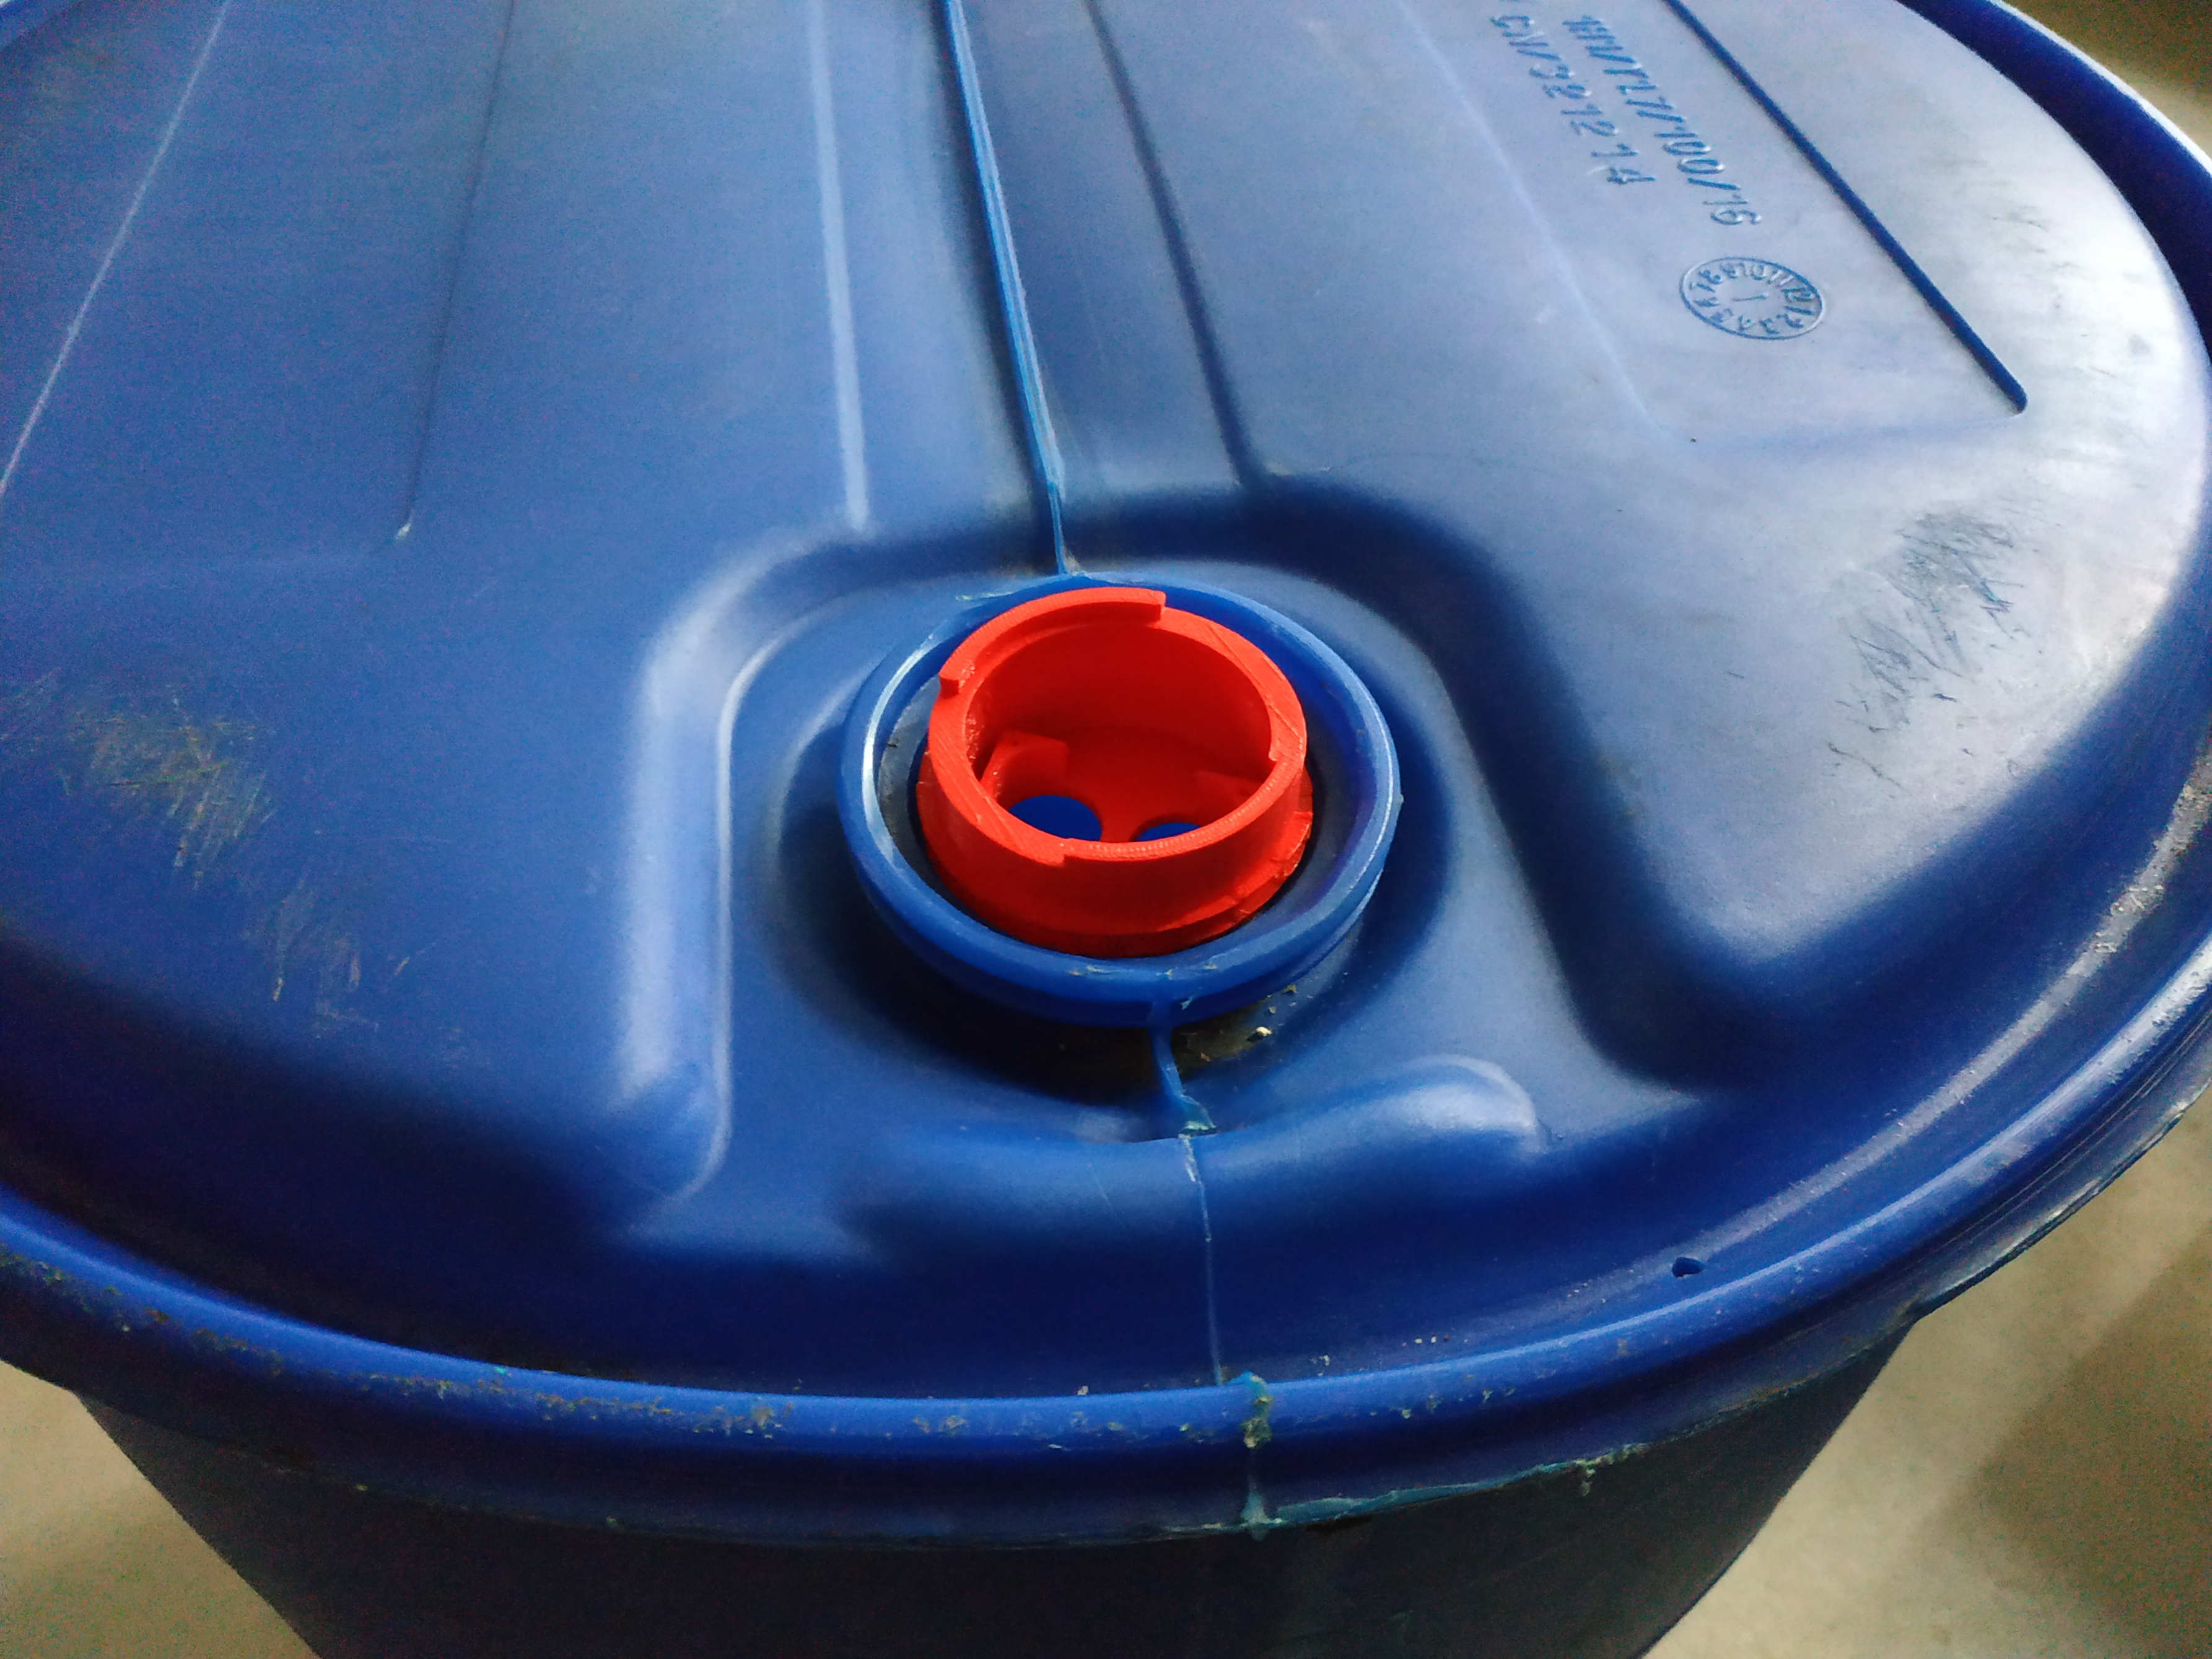
\includegraphics[scale=0.14]{images/Development/3D_device_development/screwThreadTest.pdf}
    \caption{Printed 3D screw thread being tested.}
    \label{fig:3DscrewThead}
\end{figure}

Thus, the electronic components is drawn in solid model and is used in order to have a better understanding about the dimensions and design of the whole device model. In Figure~\ref{fig:preview3Dmodell}, it is shown a preview model of the whole device. From the front view in Figure~\ref{fig:frontViewPreviewModel}, there are two access openings, one for the micro USB module charger and one for the ESP32. In the middle, it will be placed a switch button for turning the device ON and OFF. The openings from the side view, in Figure~\ref{fig:sideViewPreviewModel}, are for the ESP32 onboard \gls{LED}s, responsible for alerting if the device is powered up and for the alert system, warning in case the liquid's surface is under a predetermined value.

\begin{figure}[h!]
    \centering
    \subfigure[Front view.]{
        \includegraphics[scale=0.35]{images/Development/3D_device_development/3dFrontView.pdf}
        \label{fig:frontViewPreviewModel}
    }\quad\quad\quad\quad
    \subfigure[Side view.]{
        \includegraphics[scale=0.35]{images/Development/3D_device_development/3dSideView.pdf}
        \label{fig:sideViewPreviewModel}
    }
    \caption{Preview of the 3D device model.}
    \label{fig:preview3Dmodell}
\end{figure}

Therefore, the final version of the device is demonstrated in Figure~\ref{fig:3DmodelDevice}. As can be viewed, the device has a cover which is secured by 4 screws located at the corners. Already for the Figure~\ref{fig:positionEletronicComponents}, it is shown the position of the electronic components inside of the model.

\begin{figure}[h!]
    \centering
    \subfigure[Isometric view of the device.]{
        \includegraphics[scale=0.58]{images/Development/3D_device_development/3dFinalVersion.pdf}
        \label{fig:isometricViewDevice}
    }
    \subfigure[Position of the electronic components in the device.]{
        \includegraphics[scale=0.43]{images/Development/3D_device_development/3dFinalVersionTop.pdf}
        \label{fig:positionEletronicComponents}
    }
    \caption{Final device model.}
    \label{fig:3DmodelDevice}
\end{figure}

Now that the device model is defined, it is time for the printing process. The printer uses the Simplify3D software control, which is responsible for translating the 3D models into instructions that the printer can understand. There are a wide range of information on their website in order to have better printing results. Mainly, regarding the support structures. The printed model can be seen in Figure~\ref{fig:3dDPrintedDevice}, in which PLA (short term for Polylactic Acid) filament was used as the material for the printed model.

\begin{figure}[h!]
    \centering
    \includegraphics[scale=0.43]{images/Development/3D_device_development/PrintedModel.pdf}
    \caption{3D printed model.}
    \label{fig:3dDPrintedDevice}
\end{figure}

After all the printing process, it is time to install the electronic components inside the printed device. Following the electronic circuit schematic, as illustrated in Figure~\ref{fig:schematic_projet}, the implementation resulted is shown in Figure~\ref{fig:final3Dmodel}.

\begin{figure}[h!]
    \centering
    \subfigure{
        \includegraphics[scale=0.117]{images/Development/3D_device_development/3DPrintedModelFinal.pdf}
        \label{fig:uncovered}
    }
    \subfigure{
        \includegraphics[scale=0.09]{images/Development/3D_device_development/3DPrintedModelFinalUncover.pdf}
        \label{fig:covered}
    }
    \caption{Final version of the 3D printed device.}
    \label{fig:final3Dmodel}
\end{figure}


\section{Setting up the ESP32}\label{section:settingESP32}

In this section, it is demonstrated the software development responsible to retrieve and manage the ultrasonic measurements. The development environment used to program the ESP32 Board is the Arduino \gls{IDE}, the installation of the board in the software can be done by following the steps provided by \cite{KURNIAWAN:2019} or directly in \cite{ESPRESSIF:ESP32}. After it is established the programming tool, it is time to define the characteristics adopted for the system and the flowchart overview of how the embedded software works. 


\subsection{Software Design}

Starting with the Wi-Fi configuration, it refers to the information related to the name of the Wi-Fi network (SSID), the password and the \gls{IP} host address, responsible for allowing the connection between the client and the server, where the data will be stored. 

Analyzing the barrel characteristics, it is adopted the diameter, height and volume. As there is no mathematical model that describes exactly the geometry of the barrel, it is used the Equation~\ref{eq:totalVolume} for the volume calculation.

The alert system is responsible for emitting a light warning, by turning on an ESP32 onboard \gls{LED}, in which it will inform the managements when the barrel capacity is less then a predetermined value. The \gls{LED} will maintain its state until the capacity of the sensor is above the predetermined value.

Another feature is the check system, which is responsible for saving the old value of the distance measured, in the internal memory of the ESP32, in order to compare with the new value, before the information is sent to the database. This prevention system is important for level measurement systems, specially when the liquid level to be measured does not change quickly between two consecutive measurements. Thereby, it avoids possible nonsense values to be send to the database, by comparing them before the data to be sent.

For the environment temperature, as all reservoirs are located at centralized in a room inside the facilities of the \gls{SCMB} and, each plastic barrel has only two openings, as shown in Figure~\ref{fig:topViewBarrel}, due the material of the plastic barrel and the location where they are placed, it is assumed that the average temperature is closely to constant.

Furthermore, the system has a variable which allows to define a number of samples. This variable is responsible for the US-015 ultrasonic sensor to take successively measurements, in a short period of time, with the objective to decrease the errors from the readings. 


\subsubsection{Measurement System Flowchart}

The flowchart of the sensor readings are shown in Figure~\ref{fig:flowchartUltrasonicReadings}. It is basically responsible for retrieving, avoiding and treating the ultrasonic sensor readings, calculating and returning the distance, volume and capacity of the barrel's liquid.

\begin{figure}[h!]
    \centering
    \includegraphics[scale=0.85]{images/Development/Setting_the_ESP32/flowchart_ultrasonic_readings.pdf}
    \caption{Flowchart of the ultrasonic sensor readings.}
    \label{fig:flowchartUltrasonicReadings}
\end{figure}

This function makes the ESP32 to send a pulse to the trigger pin of the US-015 with a period of 30~\begin{math}\mu s\end{math}, than it will wait for the echo answer with a timeout of 60~ms. At this point, the time is being counted. 

If the echo exists, the system will make another process to check if the returned time value is appropriate or not. In case the time is appropriate, the system will make the distance calculation, using the Equation~\ref{eq:distanceCm}, and the result will be stored in a auxiliary vector. However, if the time value is not appropriate, the ESP32 will send a low pulse to the echo pin of the US-015 in order to reset the readings received from the echo pin, preventing the system to make new readings with the same errors, due to interference factors.

The system will make repetitively measurements until the number of samples is reached. After this point, all the measurements stored in the auxiliary vector will be added and the distance mean will be calculated. Thus, the volume and capacity is calculated with the Equations \ref{eq:liquidVolume} and \ref{eq:capacity}, respectively, and the parameters are returned from the function.


\subsubsection{System Flowchart}

Upon the completion of the software design, Figure~\ref{fig:flowchart_esp32} demonstrates the flowchart of the code written and programmed into the microcontroller, it also can be found by checking in \cite{COELHO:2019}. It begins with the initialization of the parameters presented in the previous section and the libraries necessary for the development of the program.

\begin{figure}[h!]
    \centering
    \includegraphics[scale=0.9]{images/Development/Setting_the_ESP32/flowchart_esp32.pdf}
    \caption{The system flowchart.}
    \label{fig:flowchart_esp32}
\end{figure}

The libraries used are the <Wi-FiClient.h> and the <WebServer.h>, they enable the ESP32 Board to connect with a Wi-Fi network and sending information through \gls{HTTP} request method. Following, the system defines the pin mode and, makes reads from the ultrasonic sensor module, as shown in Figure~\ref{fig:flowchartUltrasonicReadings}. Thus, the distance returned is stored in an auxiliary vector for further comparisons. Lastly, the microcontroller connects to a local Wi-Fi network.

Already inside of the infinite loop, the system will update the distance value stored at the auxiliary vector by making new readings from the sensor, then, it makes an absolute difference between the old and new values. The system will make five comparisons if the distance difference is greater than 10.00 cm. In case after this five comparisons, the system continues providing this big difference, the system will decide that this value is true and it will continue with the program flow. Otherwise, the value will be discarded and the system will be forced to do other readings, from the sensor module, in order to check if the value measured is correct.

After these strict comparisons, the system will make some basic checkup and it will print, through the serial monitor, specific alerts in case of nonsense values. Then, the system will rerun the program until a reasonable distance measurement is taken.

Starting the checkup process with the US-015 ultrasonic sensor, as it is capable of doing measurements in a range of 2~cm to 4~m, the system will print \textit{Invalid measurement!} when the distance is shorter then 2.0 cm and, for the maximum operating range of the sensor, it will be limited to the barrel's height. Thereby, in case the distance measured is greater, the sensor will print a message \textit{Connect the Sensor at the Barrel!}, as it is impossible for the system to detect a higher measurement than it is. Lastly, it is verified if the distance is a number or not, in case this function is true, it will be printed \textit{Failed to Read From the Sensor!}.

At this point, the distance measured is valid and the values of the distance, volume and capacity is ready to be sent for the database. It will blink a LED, alerting that the system took the measurements, and it is about to send the data to the database. Finally, the Alert Function will turn on the ESP32 onboard \gls{LED}, in case the capacity parameter is under a predetermined value, and the values will be printed in the serial monitor. 

Following, the client makes a request by using the GET method, which is one of the \gls{HTTP} methods used to indicate that a desired action is to be performed. The action is to communicate with an \gls{API} responsible for inserting the data in a \gls{RDBMS}. The distance, volume and capacity information are passing in the form of an entity embedded in the \gls{URL} where the database server is located.

Lastly, the ESP32 board will go into a sleep state and it will remain for a while until further measurements are required. The delay time can be set according to the application necessities.


\section{Database Development}\label{section:database}

Upon to complete the review of the whole system development, this last section approach the structure of the database, the \gls{API}s and the developed web pages \cite{COELHO:2019}. As they are hosted on server, it was chosen \textit{000webhost} services, which is a free web hosting fully-functioning with \gls{PHP} and My\gls{SQL} features. The disk space available is up to 1 GB with 10 GB of bandwidth, which is more than enough for development and testing the laundry integrated system.

The Figure~\ref{fig:databaseArchitecture} illustrates the server architecture overview. As can be seen, the \gls{API}s communicate either with the database and the Web pages, allowing the users to access the database content, dynamically and interactively, through the \gls{HTML} Web pages.
 
\begin{figure}[h!]
    \centering
    \includegraphics[scale=0.75]{images/Development/web_database/database_overview.pdf}
    \caption{Web database architecture overview.}
    \label{fig:databaArchitecture}
\end{figure}

Although the Figure~\ref{fig:databaseArchitecture} is showing only two \gls{API}s, one for inserting data in the tables and another for making readings, in practice, the structure is a little bit more complex. In order to understand how the database structure works, it is necessary to make an overview about the website flowchart and the \gls{API}s diagram.


\subsection{Website Structure Overview}

The laundry managements can access the database content by navigating through the \textit{Início, Status, Histórico, Projeções, Contacto} and \textit{Sobre}, as illustrated in Figure~\ref{fig:websiteDiagram}. The useful information, for each Web page, is provided by the \gls{PHP} \gls{API}s when requested.

\begin{figure}[h!]
    \centering
    \includegraphics[scale=0.95]{images/Development/web_database/api_flowchart.pdf}
    \caption{Website structure diagram.}
    \label{fig:websiteDiagram}
\end{figure}

The communications are done by using \gls{HTTP} protocols, mostly through the GET and POST methods. It allows a large number of clients to access the platform simultaneously and, moreover, as the \gls{HTTP} supports the content negotiation, the client and servers can negotiate the desired format for a given resource, permitting the server to provide the same \gls{URL} in different formats, like \gls{JSON}, as approached by the Section~\ref{section:clienteSide}. These features increase the efficiency, flexibility and integration of the system.

The JavaScript is embedded inside of the \textit{main} element of the web document, where it will be located some features about the website \ref{subsection:features}. As the information is being dynamically updated, the consumer may have access of the last level measurement through the \gls{DHTML} document, by which provides a lot of benefits, as preview talked in Section~\ref{section:clienteSide}. 


\subsection{Web Application Features}\label{subsection:features}

In this Subsection, it is explored some features about the Web application relative to the data acquired from the measurements. It is important to highlight that, all the graphs were developed using Google Chart \gls{API}, which is a powerful free service that creates graphical charts from user-supplied data.


\subsubsection{Início}

In \textit{Início} (Start), the client might check the actual capacity of the reservoir and the status in case the system is unloading or loaded/loading. If the system is unloading, it will calculate the time remaining for the reservoir to drain out and, it will automatically show the date and time the reservoir will be totally empty. On the other side, if the system is already loaded or loading, it will only shows the actual capacity, as there is no date to estimate of when the reservoir will be empty (see Figure~\ref{fig:estimate}).

\begin{figure}[h!]
    \centering
    \includegraphics[scale=0.65]{images/Development/web_database/inicio1.pdf}
    \caption{Informative web page about the estimate graph of when the reservoir will be empty.}
    \label{fig:estimate}
\end{figure}

This calculus is possible by using a numerical solution for root-finding called secant method. As approached by \cite{GIFLAT:2013}, the method uses two points in neighborhood of the solution to determine a new estimate value. Therefore, it is possible to implement it by using a \gls{PHP} \gls{API}, where a new estimate value of the solution \begin{math}x_{i+1}\end{math} is determined from the previous two solutions \begin{math}x_i\end{math} and \begin{math}x_{i-1}\end{math}.

\begin{equation}\label{eq:secantMethod}
    x_{i+1}=x_i - \frac{f(x_i)(x_{i-1}-x_i)}{f(x_{i-1})-f(x_i)}
\end{equation}

The algorithm from the Equation~\ref{eq:secantMethod} was applied in the \gls{API} called Secant Method, as seen in Figure~\ref{fig:websiteDiagram}. It is responsible for reading the new information from the level01 table, process the data and stores the estimate date and time values in time\_predict01 table. Thus, the information is requested through \gls{AJAX} technique.


\subsubsection{Status}

In \textit{Status} page, as shown in Figure~\ref{fig:statusLayout}, the customer has the access to the last measurement values. It is a simple interface responsible for dynamically displaying the distance, volume, capacity and date and time values. The \gls{PHP} \gls{API} liable to provide the information for this Web page, only read the last value of the level01 table. Thereby, the server's response becomes much more responsive due the short length's size of the \gls{JSON} string.

\begin{figure}[h!]
    \centering
    \includegraphics[scale=0.65]{images/Development/web_database/status1.pdf}
    \caption{Status layout.}
    \label{fig:statusLayout}
\end{figure}


\subsubsection{Histórico}

Already for the \textit{Histórico} (Historical), it was used the Bootstrap framework, which is an free and open source toolkit directed at responsive, mobile front-end web development that allows the client to navigate through the whole database content, permitting the user to sort and search all the information from the database however they want. 

Although this feature brings a lot of functionalities for the Web document, the \gls{API} responsible for that, needs to read all the information from the database at once, which makes the \gls{JSON} string, from the server's response, to be excessively large when the table has a large number of rows. Therefore, it can not be dynamically updated. The resulting interface can be seen in Figure~\ref{fig:historicTable}.

\begin{figure}[h!]
    \centering
    \includegraphics[scale=0.6]{images/Development/web_database/historico1.pdf}
    \caption{Historical table layout design and functionalities.}
    \label{fig:historicTable}
\end{figure}


\subsubsection{Projeções}

Taking a close look at \textit{Projeções} (Projections) page, it is responsible for showing the client a graph overview about the consumption of the reservoir's content. The Google Chart \gls{API} will read the last measurements from the device, this value can be configured by changing how much information the customer prefers, through the \gls{PHP} \gls{API} named \textit{Read Some Values from Level01}, shown in Figure~\ref{fig:websiteDiagram}. Although this value might be configured, it is not recommended to use a higher number as set in default, which is pre-configured for showing the last 500 measurements, due to the fact the Web page is being continuously updated via \gls{AJAX}, and it may overload the browser's cache memory, making it necessary to restart the browser in the course of time (see Figure~\ref{fig:projections}).

\begin{figure}[h!]
    \centering
    \includegraphics[scale=0.6]{images/Development/web_database/projecoes1.pdf}
    \caption{Graph design overview.}
    \label{fig:projections}
\end{figure}


\subsubsection{Contacto}

The last feature from the website is the \textit{Contacto} or Contact form, this feature allows the consumer to get in touch with the technicians, by sending to an pre-configured email address the description of the problem. It is a basic contact form that uses the POST method to request the \gls{API} to send an email using a local \textit{sendmail program}, through the \gls{PHP} function \textit{mail()}.

This feature is an integral part of any project or business, which allows a responsiveness and well-planned communication between the client and the system's responsible. The contact form layout can be seen in Figure~\ref{fig:contactForm}. 

\begin{figure}[h!]
    \centering
    \includegraphics[scale=0.5]{images/Development/web_database/contacto1.pdf}
    \caption{Contact form layout design.}
    \label{fig:contactForm}
\end{figure}


\subsubsection{Sobre}

Lastly, in \textit{Sobre} (About) page, it is presented just a static \gls{HTML} text that provides, for the client, some basic information about the project.

\subsubsection{Website Address}

The website developed can be found by accessing the following \gls{URL}: \url{https://scmb-esp32.000webhostapp.com/application/index.php}.

It is important to point out that, due to the web technologies used here, the website content may not appear correctly for everyone, as it will depends about the hardware characteristics that is being used by the user. The browser version where the website was developed is based on \textit{Firefox version 69.0.3 (64-bit)}.
\cleardoublepage
\chapter{Results and Discussions}\label{cap:results}


\section{Experimental Testing Methodology}\label{section:testingMethodology}

There were performed some tests on the the reservoirs from the \gls{SCMB} and the system integrated worked well. Although some difficulties were presented, principally due the format of the thread pitch, the 3D device model was able to fit in the openings of the plastic drum barrels, and the measurements could be taken from the detergent surface level.

In order to characterize the developed measurement system, as demonstrated in Figure~\ref{fig:flowchartUltrasonicReadings}, some experimental tests were performed with the objective of verifying the system's accuracy. For this purpose, the device was submitted to take 50 measurements from an object surface, as can been in Figure~\ref{fig:measurementTesting}, and four tests were performed with eight different distances, within a range of 5 cm to 400 cm. For each test, it was varied the filter size, which is responsible for the ultrasonic sensor to take successively measurements, in a short period of time, and to return the mean of these values.

\begin{figure}[h!]
    \centering
    \includegraphics[scale=0.075]{images/Results/testing_methodology/3Dtesting.jpg}
    \caption{Elaborate scenario for the test measurement systems.}
    \label{fig:measurementTesting}
\end{figure}

Table~\ref{table:testSummary} shows the distances and values for each test realized. It is important to point out that these tests were performed in a controlled environment where the temperature was a known factor. 

\begin{table}[h!]
    \centering
    \begin{tabular}{@{}ccc@{}}
        \toprule
        \textbf{Tests} & \textbf{Distances (cm)} & \textbf{Filter Size} \\ \midrule
        \rowcolor[HTML]{EFEFEF} 
        A & 5/10/25/50/100/200/300/400 & 1 \\
        B & 5/10/25/50/100/200/300/400 & 5 \\
        \rowcolor[HTML]{EFEFEF} 
        C & 5/10/25/50/100/200/300/400 & 20 \\ 
        D & 5/10/25/50/100/200/300/400 & 50 \\ \bottomrule
    \end{tabular}
    \caption{Summary of the experimental tests with different distances being measured.}
    \label{table:testSummary}
\end{table}


\subsection{Analysis of the Experimental Results}

The tests performed will be presented in this subsection. Due to the large quantity of information, only some of them will be provided, however, sufficient for the analysis of the results. The rest of the tests can be found in Appendix \ref{appendice1:first}.

In Figure~\ref{fig:50cmText}, it is presented the measurement results with the object placed in a distance of 50~cm from the sensor. The first thing that can be noticed is the high value of the average systematic error presented. Although it is an inherent characteristic from any measurement process, its high value is mostly influenced due to the offset adopted for the system, in which it is considered the zero point as the beginning of the device thread, and not from the ultrasonic sensor itself.

\begin{figure}[h!]
    \centering
    \includegraphics[scale=0.5]{images/Results/testing_methodology/50cm.pdf}
    \caption{Analysis \#1 with the object placed 50 cm from the sensor.}
    \label{fig:50cmText}
\end{figure}

Another important factor is the standard deviation, in which it could be noticed that, even for distances shorter than 100 cm, all tests provided low rates of the variation, indicating that the values tend to be close to the mean of the set. 

\begin{figure}[h!]
    \centering
    \includegraphics[scale=0.5]{images/Results/testing_methodology/400cm.pdf}
    \caption{Analysis \#1 with the object placed 400 cm from the sensor.}
    \label{fig:400cmText}
\end{figure}

Already for greater distances, the tests provided better results for the tests C and D, as the values from the tests A and B are spread out over the range, which proves that, successively measurements taken from the ultrasonic sensors decrease with higher numbers of collected samples. Figure~\ref{fig:400cmText} shows the test results, with the object placed in a distance of 400 cm. It can be noticed that, for the tests A and B, the values of each sample are scattered along the graph, differently than the results from the test C and D.

The Figure~\ref{fig:systematicError} presents the systematic error from all tests performed. It can be noticed that test A has demonstrated highest values, in which decrease successively until test D.

\begin{figure}[h!]
    \centering
    \includegraphics[scale=0.43]{images/Results/testing_methodology/systematicError.pdf}
    \caption{Average systematic error presented from all the experimental results (see Appendix \ref{appendice1:first}).}
    \label{fig:systematicError}
\end{figure}

Therefore, from the analysis, the test C and D has demonstrated promising results, principally for the test D, in which it has shown the lowest systematic error and standard deviation. However, everything comes with a cost and, in this case, the cost is the time that the ultrasonic sensor takes the readings. If the liquid's level surface changes while the sensor is reading, it may directly influence on the results of the measures. 

Using a digital oscilloscope, it was possible to evaluate this time value. For the test A, the time is 50 ms for each reading. Already for test B, it is around 250 ms. The test C, the value of the readings is 1.1 s and, for test D, the time is around 2.6 s. Therefore, using higher values of samples, as the ones used for the test D, may have a direct impact on the readings. As the detergent's liquid level does not change quickly, it would be affordable for this application to use the values approached by test D. However, if the readings are showing variations, it would be interesting to reduce the number of samples, in order to make the readings from the ultrasonic sensor faster.

After this set of tests, the best number of samples to be used as default, in terms of systematic error and standard deviation, is the one that is used on test D. Even for distances up to 400 cm, the system has demonstrated some good results, evidencing that the device may be used for reservoirs with higher heights.


\section{System's Reliability}\label{section:systemReliability}

This section will approach the reliability of the system, e.i., if the system is able to take the measurements, for a long period of time, without detecting fail readings. For this purpose, the device was submitted to take 1000 measures, within a range of distances from 10 cm to 90 cm. Higher values will not be considered, due to fact that the reservoirs from the \gls{SCMB} have height of 92 cm. Thus, it is performed some statistical analysis, in order to provide the system's accuracy.

In order to simplify the analysis process, it is chosen only three cases wherein the the object is placed 10 cm, 50 cm and 90 cm from the sensor, represented by Figures \ref{fig:conf10TEXT}, \ref{fig:conf50TEXT} and \ref{fig:conf90TEXT}, respectively. The rest of the results can be found in Appendix \ref{appendice1:second}. 

\begin{figure}[h!]
    \centering
    \includegraphics[scale=0.5]{images/Results/testing_methodology/conf10.pdf}
    \caption{Analysis \#2 with the object placed 10 cm from the sensor.}
    \label{fig:conf10TEXT}
\end{figure}

\begin{figure}[h!]
    \centering
    \includegraphics[scale=0.5]{images/Results/testing_methodology/conf50.pdf}
    \caption{Analysis \#2 with the object placed 50 cm from the sensor.}
    \label{fig:conf50TEXT}
\end{figure}
\clearpage
\begin{figure}[h!]
    \centering
    \includegraphics[scale=0.5]{images/Results/testing_methodology/conf90.pdf}
    \caption{Analysis \#2 with the object placed 90 cm from the sensor.}
    \label{fig:conf90TEXT}
\end{figure}

The Table~\ref{table:samples1000} presents the object distance, the mean values of the samples $\bar{x}$, the standard deviation $\sigma_s$, the systematic error $S_E$ and the relative error $\varepsilon$ of the 1000 samples taken. 

\begin{table}[h!]
    \centering
    \begin{tabular}{@{}ccccc@{}}
        \toprule
        \textbf{Distance (cm)} & \textbf{$\bar{x}$} (cm)& \textbf{$\sigma_s$} (cm) & \textbf{$S_E$} (cm) & \textbf{$\varepsilon$} (\%)\\ \midrule
        \rowcolor[HTML]{EFEFEF} 
        90 & 91.73 & 0.07 & 1.73 & 1.92 \\
        50 & 51.63 & 0.06 & 1.63 & 3.27 \\
        \rowcolor[HTML]{EFEFEF} 
        10 & 11.01 & 0.03 & 1.01 & 10.08 \\ \bottomrule
    \end{tabular}
    \caption{Summary of the result values presented from the 1000 samples collected.}
    \label{table:samples1000}
\end{table}

As can be noticed, for longer distances, the samples has demonstrated higher values of standard deviation $\sigma_s$, principally when comparing with shorter distances. This is an expected result, due to the fact the ultrasonic waves are travelling for longer distances. Taking a close look at the relative error $\varepsilon$, shorter distances have presented higher values, as the variations for small distances will have a significant impact, on the relative error, than for longer distances. 

In order to make a better assessment of the measurements, it will be selected 15 random values from the 1000 samples collected, and the system measurement will be evaluated with a confidence interval of 95~\%. As approached by \cite{NETO:2012}, measurement results $MR$ can be evaluated through the Equation~\ref{eq:measurementResult}

\begin{equation}\label{eq:measurementResult}
    MR = \bar{x} - S_E~\pm~\frac{Re}{\sqrt{n}}
\end{equation}
where $n$ is the number of samples and $Re$ is the repeatability of a measurement instrument, defined by the Equation~\ref{eq:repetitively}

\begin{equation}\label{eq:repetitively}
    Re = \pm~t~_x~\sigma_s
\end{equation}
in which t is the Student t-distribution.

Therefore, for a $n = 15$ samples, considering one degree of freedom ($n$ - 1) = 14 and 95\% of probability, from the table of t-distribution \cite{NETO:2012}, it is found that $t = 2.14$. Thereby, it is possible to find the repeatability of the system and define the measurement system results. Its results is demonstrated in Table~\ref{table:mr}.

\begin{table}[h!]
    \centering
    \begin{tabular}{@{}cccccc@{}}
        \toprule
        \textbf{Distance (cm)} & \textbf{$\bar{x}$ (cm)} & \textbf{$\sigma_s$ (cm)} & \textbf{$S_E$ (cm)} & \textbf{$Re$ (cm)} & \textbf{MR (cm)} \\ \midrule
        \rowcolor[HTML]{EFEFEF} 
        90 & 91.71 & 0.06 & 1.71 & 0.1 & 90.00 $\pm$ 0.03 \\
        50 & 51.65 & 0.07 & 1.65 & 0.1 & 50.00 $\pm$ 0.03 \\
        \rowcolor[HTML]{EFEFEF} 
        10 & 11.02 & 0.02 & 1.02 & 0.04 & 10.00 $\pm$ 0.01 \\ \bottomrule
    \end{tabular}
    \caption{Measurement system result using a confidence interval of 95 \% and a t-distribution of $t$ = 2.14 \cite{NETO:2012}.}
    \label{table:mr}
\end{table}

From the analysis, it can be noticed that, for the distances 90 and 50 cm, there are 95~\% of probability that the resultant values from the measurements would be within the range of $\pm$ 0.03 cm. Already for the distance of 10 cm, the range is shorter, presented a range of values within $\pm$ 0.01 cm. These values represent positive results, indicating that the accuracy of the measurement system, from the developed device, is in agreement for the detergent supervision application.


\section{Analysis of the Temperature Influence}\label{section:temperatureInfluence}

As it is more interesting, for the client, to know about the capacity and volume of the reservoir than the distance measured from the sensor, in this section, it will be approached the influence of the temperature on the reservoir capacity measured by the sensor, once it is not being used a temperature sensor. Also, it is important to highlight that reservoirs are kept in a close environment, so the temperature variation presented here are only for comparison effects.

Using the \textit{MATLAB} software, it was possible to evaluate the capacity variation as a function of the temperature. As can be seen in Figure~\ref{fig:test_temperature}, it is analyzed three tests with the capacity of the reservoir being at 5~\%, which is considered one of the cases where the temperature will have significant influence on the capacity measured. Thereby, for the test A, the temperature set in the ESP32 Module is 15ºC, for test B, 20ºC and for test C, 25ºC. Thus, the temperature is varied in a range of 5ºC to 35ºC.

\begin{figure}[h!]
    \centering
    \includegraphics[scale=0.55]{images/Results/temperature_influence/Analyse_5.pdf}
    \caption{Reservoir Capacity: 5 \%; Test A: 15ºC; Test B: 20ºC; Test C: 25ºC.}
    \label{fig:test_temperature}
\end{figure}

From the analysis, the best case happens when the environment temperature is the same as the one programmed at the ESP32 Module, where the device detects the exact level measurement of the reservoir. In mostly normal conditions, the variation on the capacity would be around $\pm$ 1~\%. However, when extrapolating the variation of the temperature for 35ºC, the system would detect an maximum error slightly above 3~\%. 

In Appendix \ref{appendice1:third}, it can be found others cases where it was analyzed the capacity variation with the reservoir being at 50~\% and 95~\%. The results of the variation presented was around 1~\%, for the reservoir capacity being at 50~\%, and practically null for the reservoir that is almost full.

Therefore, the temperature sensor is not so important in this kind of application, as it will have a minimum impact on the capacity measurements. Although, in applications where the variation of 1 \%, in the reservoir's capacity, is important, it would be interesting to evaluate the use of a temperature sensor.


\section{Battery Performance}\label{section:batteryPerformance}

In order to have an assessment of the battery performance, first, it is important to point out that, the time for the system to update the \textit{status} of the detergent level on the database, may differ according to the stringency criteria that the application requires. 

The time value that the sensor will take the readings, is best estimate by implementing the system on the reservoirs at the \gls{SCMB}, and evaluate the time that would provide the best conditions, both for the battery usage and, for the readings.

Therefore, it is more interesting to talk about how many measurements (readings) the system is able to make. After some practical tests, it was possible to evaluate that, the system can make readings and update the information on the database around 9300 times. If the stringency criteria of the information to be updated is high, it would be interesting to use another battery connected, in parallel, in order to make the working time of the device longer or, it is possible to use it plugged directly with a 5 V charger, with a maximum current output of 1 A.

\section{Overall Considerations}\label{section:overallConsiderations}

In this section, it will be presented some basic considerations about the solution adopted for the detergent supervision.

First, as any \gls{IoT} application, the device must be 100~\% of the time connected with a network, otherwise, the system will no longer be able to take the readings and update the information on the database. In case the internet access is not available, some adjusts can be made, with the objective of making the ESP32 Module to save the values from the readings on its internal memory and, when the internet access becomes available again, the system would update the information all at once. Although it would be an interesting solution, for the time period that the system is offline, it would not be considered a real-time monitoring solution.

The Web platform developed in this work does not make use of any \gls{API} protection. This means that the \gls{API}s may be target of security threats and, additional vulnerabilities, due to the none use of authentication and lack of encryption. Therefore, the use of Simple Object Access Protocol (SOAP) or Representational State Transfer (REST) would be interesting in order to deal with transactional massaging security considerations, principally using an authentication and authorization architecture.

Another point to be considered is regard to the environment where the device will be placed. In the laundries facilities of the \gls{SCMB}, it is used five types of products to clear the clothes, e.g., liquid detergent, chlorinated and oxygenated blancher, neutral detergent and softener. Therefore, the device must be evaluated in order to check if the environment is being aggressive for the equipment and, if the measurements is going to be affected in the course of time. 

\section{System Cost and Architecture Proposal}\label{section:systemCost}

This section will provide an overview of the price of the components used for the work development. The values of the plastic usage (PLA) for the printing process and the wiring connections will not be considered. Moreover, the services provided from the \textit{000webhost}, for the database storage, is free, although with a limit of disk usage up to 1 GB.

From the Table~\ref{table:cost}, it can be noticed that the developed integrated system provides a low-cost \gls{IoT} solution for industrial washing machines, with prices varying around 8 to 9 \euro. Due to the number of functionalities and the reliability performed from the tests analysis, it makes the product a very interesting solution for the measurement level.

\begin{table}[h!]
    \centering
    \begin{tabular}{@{}ccc@{}}
        \toprule
        \textbf{Items} & \textbf{Quantity} & \textbf{Price (\euro)} \\ \midrule
        \rowcolor[HTML]{EFEFEF} 
        ESP32 Development Kit v1 & 1 & 3.54 \\
        US-015 Ultrasonic Sensor & 1 & 0.52 \\
        \rowcolor[HTML]{EFEFEF} 
        DC-DC Boost Converter 3 V to 5 V & 1 & 0.61 \\
        03962A Li-Ion Battery Charger & 1 & 0.16 \\
        \rowcolor[HTML]{EFEFEF} 
        LIR18650 2600 mAh & 1 & 3.50 \\
        Battery Case Holder & 1 & 0.52 \\ \hline
        \rowcolor[HTML]{EFEFEF} 
        \textbf{Total} & - & \textbf{8.85} \\ \bottomrule
    \end{tabular}
    \caption{Price table of the electronic components used. \textit{Prices based on Aliexpress and eBay (October, 2019)}.}
    \label{table:cost}
\end{table}

The advantages of having a low-cost device is the scalability, as its application can be transferred for others reservoirs, making the production more flexible. Also, it will improve the efficiency of the productive process, as it can be add actuators that can pump the liquid from spare reservoirs when a low level of capacity is detected. This \gls{IoT} Ecosystem is illustrated in Figure~\ref{fig:final}, where all the reservoirs are connected with the device developed, and all the information may be accessed through different platforms.

\begin{figure}[h!]
    \centering
    \includegraphics[scale=0.13]{images/Results/modeloFinal.png}
    \caption{IoT Ecosystem for Industrial Washing Machines.}
    \label{fig:final}
\end{figure}
\cleardoublepage
\chapter{Conclusions and Future Work}\label{cap:conclusions}

The concepts of the Industry 4.0 comprises the idea of making the production more flexible, by using cutting edge technologies in order to maintain the competitive business environment. In the field of laundry industry, the necessity to ensure an effective logistics is essential to keep the quality and productivity of the service. In this context, the present work developed a solution based on \gls{IoT} to be applied in industrial washing machines. The developed integrated system demonstrated to be capable of monitoring and recording the detergent liquid level in a web database, allowing the laundries management to access the measurement results through a web platform.

To implement the system in the reservoirs, the printed device model evidenced to be efficient, as it provides a good positioning, for the ultrasonic sensor, to take the readings from the detergent liquid surface. Furthermore, it performs a very simply and compact solution, as it allows the measurements to be collected without being necessary to make modifications on the reservoir's structure, making it an attractive differential for the adopted solution. The analysis results from the measurements indicated that the use of low-cost ultrasonic sensor is very appropriate for this application, as the failed readings could be treaties, with the use of an embedded system, providing very good accuracy of the measurements. Also, the developed device proved promising to be used for reservoirs with heights up to 400 cm. For the web database connection, the use of \gls{PHP} \gls{API}s demonstrated to be efficient, being able to read large amounts of data from the database without compromising the user experience, however, security threats may be a problem due to the none use of authentication and lack of encryption. Finally, the use of \gls{AJAX} technique provides a wealth combination with the \gls{IoT} solution adopted, enabling the Web document to be dynamically displayed through the \gls{DHTML} web pages.

In general, there are several ways to perform level measurements and it represents an important indicator for process control. The use of direct methods may be simpler than the indirect ones, however, it may not be suitable for automated control. The non-contact level measurement using ultrasonic sensor, embedded alongside with a microcontroller, demonstrated to be affordable as a part of \gls{IoT} solution for industrial washing machines. Besides the detergent liquid level, the solution developed here may be applied for others liquids, since it does not have dynamic changes.

For the future works, it is expected the system to be implemented, in the laundry facilities of the \gls{SCMB}, with the objective to be tested others parameters, especially regarding the durability of the developed device, i.e., to check if the environment is damaging, in the course of time, the electronic components and/or the PLA material. Moreover, another important criterion is the implementation of \gls{API} protection, such as REST and SOAP, which must be developed for the work advancement.

%% estilo de referências. outros valores posíveis são 'plain' e 'abbrv' apalike
%\bibliographystyle{plain}
%% listagem de referências
%\bibliography{lib/refs}

%  Caso seja usado biblatex
\printbibliography

% Apêndices
\appendix

%http://tex.stackexchange.com/questions/59572/custom-page-numbering-for-appendix
\pretocmd{\chapter}{%
	\clearpage
	\pagenumbering{arabic}%
	\renewcommand*{\thepage}{\thechapter\arabic{page}}%
}{}{}

\chapter{Publications}\label{apendice3}

\subsection*{Paper Submitted and Accepted}

Coelho, G. G., Coelho, J. P., \& Moretti, E. H. (2019). Development of an IoT Solution for Detergent Supervision in Industrial Washing Machines. \textit{Carpathian Journal of Electronic and Computer Engineering, 12}(2).
\input{chapters/apendice01}
\chapter{Summary of the Technical Drawings and Developed Codes}
\label{apendice2}

In this appendix, the Section~\ref{appendice:technicalDrawings} illustrates the technical drawings regarding the development of the 3D device through the SolidWorks software.

Already, for the Section~\ref{appendice:code}, it provides the link for the GitHub, where the user can find the documents developed. The files are divided as follows:

\begin{itemize}
    \item The \textit{api} file contain all the Appication Program Interface developed using PHP programming language.
    \item Already for the \textit{application} file, it gives the access to the Front End application, where can be found the HTML/CSS and JavaScript codes.
    \item In \textit{esp32\_code} file, it is found the code structure developed using Arduino IDE in C programming language.
\end{itemize}




\clearpage
\section{Technical Drawings}\label{appendice:technicalDrawings}

\begin{figure}[h!]
    \centering
    \includegraphics[scale=0.65]{images/Results/3D_Model_Technical_Drawing.PDF}
    \caption{Technical drawing of the 3D printed model.}
    \label{fig:3dModel}
\end{figure}

\begin{figure}[h!]
    \centering
    \includegraphics[scale=0.65]{images/Results/3D_Model_Cover_Technical_Drawing.PDF}
    \caption{Technical drawing of the 3D printed cover model.}
    \label{fig:3dModelCover}
\end{figure}

\clearpage
\section{Developed Codes}\label{appendice:code}

\begin{center}
    Link for GitHub, where can be found the files with the codes applied:
\end{center}

\begin{center}
\url{https://github.com/gustavogoncalvescoelho/IoT-Solution-For-Industrial-Washing-Machines}
\end{center}


\end{document}
